\documentclass{Note}
\usepackage{amsmath} %% for equation edit
\usepackage{amsfonts} %% for equation edit
\usepackage{ulem} %sout
\usepackage{amssymb}
\usepackage{graphicx}






\begin{document}
\title{Note:Governing Euqations of General 3D duct flow} 
%%% first author
\author{
     Email: jiaqi\_wang@sjtu.edu.cn
    } 

\maketitle

\section{Hard-walled cylinderical ducts as basis function}
\subsection{Infinite straight duct mode}
We began from the Helmholtz equation:


\begin{equation}
\begin{aligned}
\nabla^2 \psi={1\over r}{\partial \over \partial  r}({ r{\partial \psi\over \partial  r}}) +{1\over  r^2}{\partial ^2 \psi \over \partial \theta^2}=-\alpha^2 \psi
\end{aligned}
\end{equation}

Using separation of variables, Circular symmetry: modes have the from :
$\psi=F(r)G(\theta)$,

Then we have:


\begin{equation}
\begin{aligned}
({\partial^2 F\over \partial r^2}+{1\over r}{\partial F\over \partial r})G+{F\over r^2}{\partial^2 G\over \partial \theta^2}=-\alpha^2 FG\\
Then,\\
{({\partial^2 F\over \partial r^2}+{1\over r}{\partial F\over \partial r})\over F}+{1\over r^2}{{\partial^2 G\over \partial \theta^2}\over G}=-\alpha^2 \\
\end{aligned}
\end{equation}

We assume that:


Due to periodicity, we require that $\Phi$ satisfy, 
\begin{equation}
\begin{aligned}
{d^2 G\over d\theta^2}=-m^2 G\rightarrow \Phi(\theta)=e^{\pm i m \theta}
\end{aligned}
\end{equation}


Thus, we  have
\begin{equation}
\begin{aligned}
F''+{1\over r} F'+(\alpha^2-{m^2\over r^2})=0  \rightarrow F(r)=J_m(\alpha r)
\end{aligned}
\end{equation}

Circular symmetry $\psi=F(r)G(\theta)$: modes explicitly given by:
\begin{equation}
\begin{aligned}
\psi=J_m(\alpha_{m\mu} r)e^{\pm i m \theta}
\end{aligned}
\end{equation}

Hard walls:
\begin{equation}
\begin{aligned}
J_m'(\alpha R)=0 \rightarrow \alpha_{m\mu}={{j'_{m\mu}}\over R}
\end{aligned}
\end{equation}

Soft walls without flow:
\begin{equation}
\begin{aligned}
Z\alpha_{m\mu} J_m'(\alpha_{m\mu} R)=-iw\rho_0J_m(\alpha_{m\mu} R) \rightarrow \alpha_{m\mu}(Z)
\end{aligned}
\end{equation}

Soft walls with flow:
\begin{equation}
\begin{aligned}
Z\alpha_{m\mu} J_m'(\alpha_{m\mu} R)=(w-U_0\kappa_{m\mu})J_m(\alpha_{m\mu} R) \rightarrow \alpha_{m\mu}(Z)
\end{aligned}
\end{equation}

A complete solution may be writtern as:
\begin{equation}
\begin{aligned}
p(x,r,\theta)=\sum_{m=-\infty}^\infty \sum_{\mu=1}^\infty (A_{m\mu}e^{-i\kappa_{m\mu}x}+B_{m\mu}e^{i\kappa_{m\mu}x})U_{m\mu}(r)e^{im\phi}\\
\end{aligned}
\end{equation}

In a hard-walled duct $U_{m\mu}e^{-im\theta}$ are orthogonal. Normalise such that:

\begin{equation}
\begin{aligned}
\int_0^{2\pi}\int_0^R U_{m\mu}(r)e^{-im\theta}U_{nv}(r)e^{-in\theta}rdr=2\pi \delta_{\mu v}\delta_{mn}
\end{aligned}
\end{equation}

Source expansion
If $p(0,t,\theta)=p_0(r,\theta)$ is source in hard-walled duct, then for x>0
\begin{equation}
\begin{aligned}
p_0(r,\theta)=\sum_{m=-\infty}^\infty \sum_{\mu=1}^\infty (A_{m\mu}e^{-i\kappa_{m\mu}0})U_{m\mu}(r)e^{-im\theta}\\
p_0(r,\theta)\underline{U_{nv}(r)e^{-in\theta}r}=\sum_{m=-\infty}^\infty \sum_{\mu=1}^\infty (A_{m\mu}e^{-i\kappa_{m\mu}0})U_{m\mu}(r)e^{-im\theta}\underline{U_{nv}(r)e^{-in\theta}r}\\
\underline{\int_0^{2\pi}\int_0^R} p_0(r,\theta)\underline{U_{nv}(r)e^{-in\theta}r}\underline{drd\theta}=\underline{\int_0^{2\pi}\int_0^R}\sum_{m=-\infty}^\infty \sum_{\mu=1}^\infty (A_{m\mu}e^{-i\kappa_{m\mu}0})U_{m\mu}(r)e^{-im\theta}\underline{U_{nv}(r)e^{-in\theta}r}\underline{drd\theta}\\
\underline{\int_0^{2\pi}\int_0^R} p_0(r,\theta)\underline{U_{nv}(r)e^{-in\theta}r}\underline{drd\theta}=\sum_{m=-\infty}^\infty \sum_{\mu=1}^\infty A_{m\mu}\underline{\int_0^{2\pi}\int_0^R}U_{m\mu}(r)e^{-im\theta}\underline{U_{nv}(r)e^{-in\theta}r}\underline{drd\theta}\\
A_{nv}={1\over 2\pi}\underline{\int_0^{2\pi}\int_0^R} p_0(r,\theta)\underline{U_{nv}(r)e^{-in\theta}r}\underline{drd\theta}
\end{aligned}
\end{equation}
and $B_{nv}=0$. The same for $x<0$ with $A_{nv}$ and $B_{nv}$ interchanged.

A finite number of modes (cut-on modes) survive at large distrances.
Just 1 mode if kR<<1: only $A_{01}$ important.


\subsection{General duct mode}
The pressure and velocity can now be expressed as Fourier series. Upper indices shall be used to denote temporal decompositions:

\begin{equation}
\begin{aligned}
\widehat{p}=\sum_{a=-\infty}^{\infty}P^a(\textbf{x})e^{-iawt}\\
\widehat{u}=\sum_{a=-\infty}^{\infty}U^a(\textbf{x})e^{-iawt}\\
\widehat{v}=\sum_{a=-\infty}^{\infty}V^a(\textbf{x})e^{-iawt}\\
\widehat{w}=\sum_{a=-\infty}^{\infty}W^a(\textbf{x})e^{-iawt}\\
\end{aligned}
\end{equation}

\begin{equation}
\begin{aligned}
P^a=\sum_{\alpha=0}^{\infty}P_{\alpha_{m\mu}}^a(s)\psi_{\alpha_{m\mu}} (s,r,\theta)=\sum_{m=-\infty}^\infty \sum_{\mu=1}^\infty P_{\alpha_{m\mu}}^a(s)\psi_{\alpha_{m\mu}}(s,r,\theta)\\
U^a=\sum_{\alpha=0}^{\infty}U_{\alpha_{m\mu}}^a(s)\psi_{\alpha_{m\mu}} (s,r,\theta)=\sum_{m=-\infty}^\infty \sum_{\mu=1}^\infty U_{\alpha_{m\mu}}^a(s)\psi_{\alpha_{m\mu}}(s,r,\theta)\\
V^a=\sum_{\alpha=0}^{\infty}V_{\alpha_{m\mu}}^a(s)\psi_{\alpha_{m\mu}} (s,r,\theta)=\sum_{m=-\infty}^\infty \sum_{\mu=1}^\infty V_{\alpha_{m\mu}}^a(s)\psi_{\alpha_{m\mu}}(s,r,\theta)\\
W^a=\sum_{\alpha=0}^{\infty}W_{\alpha_{m\mu}}^a(s)\psi_{\alpha_{m\mu}} (s,r,\theta)=\sum_{m=-\infty}^\infty \sum_{\mu=1}^\infty W_{\alpha_{m\mu}}^a(s)\psi_{\alpha_{m\mu}}(s,r,\theta)\\
\end{aligned}
\end{equation}




\subsubsection{Discussion of property of $\psi$}
In Jams's thesis, $\psi_\alpha=C_{\alpha_{m\mu}}J_m({{j'}_{m\mu} r\over h})cos(m\phi-\xi\pi/2)$.As he mentioned, it was merely a matter of preference  - I find it easier to visualise the modes as being "symmetric" and "anti-symmetric" along the plane of torsion free ducts, but the other method is equally as valid. 

However, there still a problem, which may cause error, but is not mentioned in the thesis:\\
\begin{equation}
\begin{aligned}
\int_0^{2\pi} cos(m\phi-\xi\pi/2)^2 d\theta={1+cos(2m\phi-\xi \pi)\over 2}|_0^{2\pi}=\left\{\begin{matrix}
\pi,m\neq 0\\
2\pi,m=0,\xi=0\\
0,m=0,\xi=1
\end{matrix}\right.
\end{aligned}
\end{equation}

In the note, we try to introduce the common solution of $\psi$ may have the form the same as the hard walls modes:
\begin{equation}
\begin{aligned}
\psi_{m\mu}(r)=C_{\alpha_{m\mu}}J_m({{j'}_{m\mu} r\over h})e^{im\phi}
\end{aligned}
\end{equation}

where may be normalized according to:
\begin{equation}
\begin{aligned}
\int_0^{2\pi}\int_0^h \psi_{\alpha_{m\mu}} \psi_{\beta_{nv}} r dr d\theta=\delta_{\mu v} \delta_{mn}
\end{aligned}
\end{equation}


In fact, we know that:
\begin{equation}
\begin{aligned}
\int_0^{2\pi} e^{im\phi}e^{im\phi}  d\theta=0\\
\int_0^{2\pi} e^{im\phi}e^{-im\theta}  d\theta=2\pi\\
\end{aligned}
\end{equation}


The orthogonality relation of Bessel function, with $J_{-m}(z)=(-1)^m J_m(z)$
\begin{equation}
\begin{aligned}
\int_0^h r J_m({{j'}_{m\mu} r\over h})J_m({{j'}_{mv} r\over h}) dr=0,\mu\neq v\\
\int_0^h r J_m({{j'}_{m\mu} r\over h})J_{-m}({{j'}_{-mv} r\over h}) dr\\=(-1)^m \int_0^h r J_m({{j'}_{m\mu} r\over h})J_{m}({{j'}_{mv} r\over h}) dr=0,\mu\neq v\\
\end{aligned}
\end{equation}

That changes our idea of normalization to:


\begin{equation}
\begin{aligned}
\uuline{\int_0^{2\pi}\int_0^h \psi_{\alpha_{m\mu}} \psi_{\beta_{nv}} r dr d\theta=(-1)^m\delta_{\mu v} \delta_{m,-n}}
\end{aligned}
\end{equation}



\subsection{Normalised Modes$\rightarrow C_{\alpha_{m\mu}}$}


Relation involving intergrals:
\begin{equation}
\begin{aligned}
\underline{2\int \alpha^2 x J_m(\alpha x)^2 dx=(\alpha^2x^2-m^2)J_m(\alpha x)^2+\alpha^2 x^2 J'_m(\alpha x)^2}\\
\rightarrow 2\int_0^h \alpha^2 x J_m(\alpha x)^2 dx=[(\alpha^2x^2-m^2)J_m(\alpha x)^2+\alpha^2 x^2 J'_m(\alpha x)^2]|_0^h\\=[(\alpha^2x^2-m^2)J_m(\alpha x)^2+\alpha^2 x^2 J'_m(\alpha x)^2]|_h-[(\alpha^2x^2-m^2)J_m(\alpha x)^2+\alpha^2 x^2 J'_m(\alpha x)^2]|_0\\
=[(\alpha^2h^2-m^2)J_m(\alpha h)^2+\alpha^2 h^2 J'_m(\alpha h)^2]-[(\alpha^2 0^2-m^2)J_m(\alpha 0)^2+\alpha^2 0^2 J'_m(\alpha 0)^2]\\
=
(\alpha^2h^2-m^2)J_m(\alpha h)^2+\alpha^2 h^2 J'_m(\alpha h)^2
\end{aligned}
\end{equation}

With hard-walled boudary condition:
\begin{equation}
\begin{aligned}
J_m'(\alpha h)=0 \rightarrow \alpha_{m\mu}={{j'_{m\mu}}\over h} (eigenvalues)
\end{aligned}
\end{equation}

Then, we have(ref: Rienstra-Fundamentals of Duct Acoustics-(55)):
\begin{equation}
\begin{aligned}
\int_0^h  r J_m(\alpha r)  J_{-m}(\alpha r)dr=(-1)^m\int_0^h  r J_m(\alpha r)^2 dr\\
=(-1)^m 
{1\over 2\alpha_{m\mu}^2}(\alpha_{m\mu}^2h^2-m^2)J_m(\alpha_{m\mu} h)^2\\
=(-1)^m 
({J_m(\alpha_{m\mu} h)\sqrt{(h^2-{m^2\over \alpha_{m\mu}^2} )}\over \sqrt{2}})^2\\
=(-1)^m 
({{h^2\over 2}(1-{m^2\over {j'}_{m\mu}^2} )}J^2_m({j'}_{m\mu}))\\
\end{aligned}
\end{equation}

Thus, with $\int_0^{2\pi} e^{im\phi}e^{-im\theta}  d\theta=2\pi$,
$\psi_{\alpha_{m\mu}}(r)=C_{\alpha_{m\mu}}J_m({{j'}_{m\mu} r\over h})e^{im\phi}$,we have:
\begin{equation}
\begin{aligned}
C_{\alpha_{m\mu}}={i^m\over \sqrt{({{\pi h^2}(1-{m^2\over {j'}_{m\mu}^2} )}J^2_m({j'}_{m\mu}))}}\\
except for:
C_{\alpha_{01}}={1 \over \sqrt{\pi}h}
\end{aligned}
\end{equation}

for 
 $\int_0^{2\pi}\int_0^h \psi_{\alpha_{m\mu}} \psi_{\beta_{nv}} r dr d\theta=\delta_{\mu v} \delta_{m,-n} =\widehat{\delta }_{\alpha\beta}=I$.


\subsection{Slowly varying ducts}

waiting for updating......

\subsection{Orthogonal-eigenvector}
 ref:https:\\www.mathworks.com/help/matlab/ref/eigs.html
 
 Eigenvectors, returned as a matrix. The columns in V correspond to the eigenvalues along the diagonal of D. The form and normalization of V depends on the combination of input arguments:

[V,D] = eigs(A) returns matrix V, whose columns are the eigenvectors of A such that A*V = V*D. The eigenvectors in V are normalized so that the 2-norm of each is 1.

If A is symmetric, then the eigenvectors, V, are orthonormal.

[V,D] = eigs(A,B) returns V as a matrix whose columns are the generalized eigenvectors that satisfy A*V = B*V*D. The 2-norm of each eigenvector is not necessarily 1.

If B is symmetric positive definite, then the eigenvectors in V are normalized so that the B-norm of each is 1. If A is also symmetric, then the eigenvectors are B-orthonormal.

We could further study this question!!

if we can use the GramSchmidt mode as basis??

\section{Mass equation}

Mass consevation:
\begin{equation}
-ia\kappa P^a+\nabla\cdot \textbf{U}^a=\sum_{b=-\infty}^{+\infty}(-P^{a-b} \nabla \cdot \textbf{U}^b-\textbf{U}^{a-b}  \cdot \nabla P^b- {B\over {2A}}iakP^bP^{a-b})
\end{equation}

First, derivation of eq1:

We know that:
\begin{equation}
h_s=1-\kappa r cos(\phi),
h_r=1,
h_\theta=r
\end{equation}

Then,
\begin{equation}
\begin{aligned}
\nabla \cdot \textbf{U}^a={1\over{h_1 h_2 h_3}}[{\partial(v_1 h_2 h_3)\over \partial w_1}+{\partial(v_2 h_3 h_1)\over \partial w_2}+{\partial(v_3 h_1 h_2)\over \partial w_3}] \\
={1\over r(1-\kappa r cos(\phi))} [{\partial(U^a r)\over \partial s}+{\partial(V^a r(1-\kappa r cos(\phi)))\over \partial r}+{\partial(W^a (1-\kappa r cos(\phi)))\over \partial \theta}]
\end{aligned}
\end{equation}

Thus, we have the mass equation,  approximate RHS by:
\begin{equation}
\begin{aligned}
\nabla \cdot \textbf{U}^b=ib\kappa P^b+o(M^2)\\
\nabla P^b=ib\kappa \textbf{U}^b+o(M^2)
\end{aligned}
\end{equation}

 Then we have
\begin{equation}
\begin{aligned}
-ia\kappa P^a+{1\over r(1-\kappa r cos(\phi))} [{\partial(U^a r)\over \partial s}+{\partial(V^a r(1-\kappa r cos(\phi)))\over \partial r}+{\partial(W^a (1-\kappa r cos(\phi)))\over \partial \theta}]\\
=\sum_{b=-\infty}^{+\infty}(-ib\kappa P^{a-b} P^{b} -ib\kappa U^{a-b} U^{b}-ib\kappa V^{a-b} V^{b}-ib\kappa W^{a-b} W^{b}  - {B\over {2A}}iakP^bP^{a-b})
\end{aligned}
\end{equation}

The fourier harmonics are expanded as follows:
\begin{equation}
\begin{aligned}
P^a=\sum_{\beta=0}^\infty P_\beta^a (s) \psi_\beta(s,r,\theta)\\
U^a=\sum_{\beta=0}^\infty U_\beta^a (s) \psi_\beta(s,r,\theta)\\
V^a=\sum_{\beta=0}^\infty V_\beta^a (s) \psi_\beta(s,r,\theta)\\
W^a=\sum_{\beta=0}^\infty W_\beta^a (s) \psi_\beta(s,r,\theta)
\end{aligned}
\end{equation}

with normalized relation:
\begin{equation}
\begin{aligned}
\int_0^{2\pi}\int_0^h \psi_\alpha\psi_\beta r dr d\theta=\widehat{\delta }_{\alpha\beta}
\end{aligned}
\end{equation}

Reorganize the eq5:
\begin{equation}
\begin{aligned}
-ia\kappa P^a(1-\kappa r cos(\phi))+{1\over r} {\partial(U^a r)\over \partial s}+{1\over r}{\partial(V^a r(1-\kappa r cos(\phi)))\over \partial r}+{1\over r}{\partial(W^a (1-\kappa r cos(\phi)))\over \partial \theta}\\
=(1-\kappa r cos(\phi))\sum_{b=-\infty}^{+\infty}(-ib\kappa P^{a-b} P^{b} -ib\kappa U^{a-b} U^{b}-ib\kappa V^{a-b} V^{b}-ib\kappa W^{a-b} W^{b}  - {B\over {2A}}iakP^bP^{a-b})
\end{aligned}
\end{equation}


Intergal and insert eq 6, 7 into eq 8:

1. the first term:
\begin{equation}
\begin{aligned}
\int_0^{2\pi}\int_0^h \psi_\alpha r [-ia\kappa (1-\kappa r cos(\phi))P^a] dr d\theta\\
=-ia\kappa \sum_{\beta=0}^\infty \int_0^{2\pi}\int_0^h \psi_\alpha\psi_\beta r [(1-\kappa r cos(\phi))] dr d\theta P_\beta^a\\
\Rightarrow -ia \kappa \Psi_{\alpha\beta}[r(1-\kappa cos(\phi))] P_\beta^a \\
(summation convention)
\end{aligned}
\end{equation}

2. the second term:

From 1.1 as example, we know that
\begin{equation}
\begin{aligned}
\int_0^{2\pi}\int_0^h   {{\partial }\over {\partial s}}[ {r U^{a-b}} U^b\psi_\alpha] dr d\theta \\
={{\partial }\over {\partial s}}\int_0^{2\pi}\int_0^h   [ {r U^{a-b}} U^b\psi_\alpha] dr d\theta 
-\int_0^{2\pi}{dh(s)\over ds}[ {r U^{a-b}} U^b\psi_\alpha]_{r=h}d\theta\\
\end{aligned}
\end{equation}

\begin{equation}
\begin{aligned}
{d\over d\alpha}(\int_{a(\alpha)}^{b(\beta)}f(x,\alpha)dx)-0+{da(\alpha)\over d\alpha}f(a(\alpha),\alpha)=\int_{a(\alpha)}^{b(\beta)}{\partial \over \partial \alpha}f(x,\alpha)dx
\end{aligned}
\end{equation}

\begin{equation}
\begin{aligned}
\int_0^{2\pi}\int_0^h \psi_\alpha r [{1\over r} {\partial(U^a r)\over \partial s}] dr d\theta\\
=\sum_{\beta=0}^\infty  \int_0^{2\pi}\int_0^h \psi_\alpha r{\partial( \psi_\beta U_\beta^a)\over \partial s} dr d\theta \\
=\int_0^{2\pi}\int_0^h \psi_\alpha \psi_\beta r{\partial( U_\beta^a )\over \partial s} dr d\theta +\int_0^{2\pi}\int_0^h \psi_\alpha r{\partial( \psi_\beta )\over \partial s} dr d\theta U_\beta^a\\
=\int_0^{2\pi}\int_0^h {\partial \psi_\alpha \psi_\beta r U_\beta^a \over \partial s} dr d\theta
-\int_0^{2\pi}\int_0^h {\partial \psi_\alpha \psi_\beta r  \over \partial s}U_\beta^a dr d\theta\\
+\int_0^{2\pi}\int_0^h  r{\partial( \psi_\alpha \psi_\beta )\over \partial s} dr d\theta U_\beta^a
-\int_0^{2\pi}\int_0^h \psi_\beta   r{\partial( \psi_\alpha )\over \partial s} dr d\theta U_\beta^a\\
=\sum_{\beta=0}^\infty  {{\partial }\over {\partial s}}\int_0^{2\pi}\int_0^h   [ \psi_\alpha \psi_\beta r U_\beta^a] dr d\theta 
-\sum_{\beta=0}^\infty  \int_0^{2\pi}{dh(s)\over ds}[ \psi_\alpha \psi_\beta r U_\beta^a]_{r=h}d\theta\\
-\sum_{\beta=0}^\infty  \int_0^{2\pi}\int_0^h   {\partial( \psi_\alpha )\over \partial s}\psi_\beta r dr d\theta U_\beta^a\\
\Rightarrow {d \over d s}(U_\beta^a \widehat{\delta }_{\alpha\beta})+0(periodic)-\Psi_{\{\alpha\}\beta}[r]U_\beta^a
\end{aligned}
\end{equation}

mark:0(periodic),which is similar in the follow momentum equation, but not eliminate in time.

3. the third term:
\begin{equation}
\begin{aligned}
\int_0^{2\pi}\int_0^h \psi_\alpha r [{1\over r}{\partial(V^a r(1-\kappa r cos(\phi)))\over \partial r}] dr d\theta\\
=\sum_{\beta=0}^\infty \int_0^{2\pi}\int_0^h \psi_\alpha {\partial(\psi_\beta r(1-\kappa r cos(\phi)))\over \partial r} dr d\theta V_\beta^a\\
=\int_0^{2\pi}\int_0^h {\partial(\psi_\alpha  \psi_\beta r(1-\kappa r cos(\phi)))\over \partial r}dr d\theta V_\beta^a-\int_0^{2\pi}\int_0^h\psi_\beta  r(1-\kappa r cos(\phi)){\partial(\psi_\alpha  )\over \partial r} dr d\theta V_\beta^a\\
=0(periodic)-\Psi_{[\alpha]\beta}[ r(1-\kappa r cos(\phi))]V_\beta^a
\end{aligned}
\end{equation}

4. the fourth term:
\begin{equation}
\begin{aligned}
\int_0^{2\pi}\int_0^h \psi_\alpha r [{1\over r}{\partial(W^a (1-\kappa r cos(\phi)))\over \partial \theta}] dr d\theta\\
=\sum_{\beta=0}^\infty \int_0^{2\pi}\int_0^h \psi_\alpha  [{\partial(\psi_\beta (1-\kappa r cos(\phi)))\over \partial \theta}] dr d\theta W_\beta^a\\
=\int_0^{2\pi}\int_0^h  [{\partial(\psi_\alpha  \psi_\beta (1-\kappa r cos(\phi)))\over \partial \theta}] dr d\theta W_\beta^a
-\int_0^{2\pi}\int_0^h  \psi_\beta (1-\kappa r cos(\phi))[{\partial(\psi_\alpha )\over \partial \theta}] dr d\theta W_\beta^a\\
=\int_0^h  [\psi_\alpha  \psi_\beta (1-\kappa r cos(\phi))]_0^{2\pi} dr W_\beta^a
-\int_0^{2\pi}\int_0^h  \psi_\beta (1-\kappa r cos(\phi))[{\partial(\psi_\alpha )\over \partial \theta}] dr d\theta W_\beta^a\\
=0-\Psi_{(\alpha)\beta}[ (1-\kappa r cos(\phi))]W_\beta^a
\end{aligned}
\end{equation}


5. the RHS term:
\begin{equation}
\begin{aligned}
\int_0^{2\pi}\int_0^h \psi_\alpha r [(1-\kappa r cos(\phi))\sum_{b=-\infty}^{+\infty}(-ib\kappa P^{a-b} P^{b} -ib\kappa U^{a-b} U^{b}-ib\kappa V^{a-b} V^{b}-ib\kappa W^{a-b} W^{b}  - {B\over {2A}}iakP^bP^{a-b})] dr d\theta\\
=\sum_{\beta=0}^{\infty} \sum _{\gamma=0}^{\infty} \int_0^{2\pi}\int_0^h \psi_\alpha \psi_\beta \psi_\gamma r  (1-\kappa r cos(\phi)) drd\theta \\  \sum_{b=-\infty}^{+\infty}(-ib\kappa P_\beta^{a-b} P_\gamma^{b}-ib\kappa U_\beta^{a-b} U_\gamma^{b}-ib\kappa V_\beta^{a-b} V_\gamma^{b}-ib\kappa  W_\beta^{a-b} W_\gamma^{b}-ia\kappa  {B\over {2A}}P_\beta^{a-b}P_\gamma^{b})\\
=\sum_{\beta=0}^{\infty} \sum _{\gamma=0}^{\infty} \Psi_{\alpha\beta\gamma}[r(1-\kappa r cos(\phi))] \sum_{b=-\infty}^{+\infty}(-ib\kappa P_\beta^{a-b} P_\gamma^{b}-ib\kappa U_\beta^{a-b} U_\gamma^{b}-ib\kappa V_\beta^{a-b} V_\gamma^{b}-ib\kappa  W_\beta^{a-b} W_\gamma^{b}-ia\kappa  {B\over {2A}}P_\beta^{a-b}P_\gamma^{b})\\
\end{aligned}
\end{equation}

Finally, we obtain the mass equation in the form of eigenfunction, the idea is same as Galerkin method:

\begin{equation}
\begin{aligned}
{d U_\beta^a \over d s}\widehat{\delta }_{\alpha\beta}-\Psi_{\{\alpha\}\beta}[r]U_\beta^a-ia \kappa \Psi_{\alpha\beta}[r(1-\kappa cos(\phi))] P_\beta^a -\Psi_{[\alpha]\beta}[ r(1-\kappa r cos(\phi))]V_\beta^a-\Psi_{(\alpha)\beta}[ (1-\kappa r cos(\phi))]W_\beta^a\\
=\Psi_{\alpha\beta\gamma}[r(1-\kappa r cos(\phi))] \sum_{b=-\infty}^{+\infty}(-ib\kappa P_\beta^{a-b} P_\gamma^{b}-ib\kappa U_\beta^{a-b} U_\gamma^{b}-ib\kappa V_\beta^{a-b} V_\gamma^{b}-ib\kappa  W_\beta^{a-b} W_\gamma^{b}-ia\kappa  {B\over {2A}}P_\beta^{a-b}P_\gamma^{b})\\
\end{aligned}
\end{equation}

\section{Momentum equation}


Momentum consevation:
\begin{equation}
-ia\kappa \textbf{U}^a+\nabla P^a=\sum_{b=-\infty}^{\infty}(-\textbf{U}^{a-b}\cdot \nabla \textbf{U}^b+P^{a-b}\nabla P^b)
\end{equation}

First, we know that
\begin{equation}
\begin{aligned}
\nabla P^a=\sum_i{1\over h_i}{\partial f\over {\partial  w_i}}\hat{h}_i={1\over {1-\kappa rcos\phi}}{\partial P^a\over {\partial s}}\hat{e}_s+{\partial P^a\over {\partial r}}\hat{e}_r+{1\over r}{\partial P^a\over {\partial \theta}}\hat{e}_\theta
\end{aligned}
\end{equation}

The RHS term is a bit complex, with the divergence of a vector U with its gradient, with

First, we know that
\begin{equation}
\begin{aligned}
(\textbf{v}\cdot \nabla )\textbf{v}^b=
\left\{\begin{matrix}
term1:\mathcal{D}v_1^b+{v_2^b\over{h_2h_1}}(v_1{{\partial h_1}\over {\partial \xi_2}}-v_2{{\partial h_2}\over {\partial \xi_1}})+{v_3^b\over{h_3h_1}}(v_1{{\partial h_1}\over {\partial \xi_3}}-v_2{{\partial h_3}\over {\partial \xi_1}})\\
term2:\mathcal{D}v_2^b+{v_3^b\over{h_3h_2}}(v_2{{\partial h_2}\over {\partial \xi_3}}-v_3{{\partial h_3}\over {\partial \xi_2}})+{v_1^b\over{h_1h_2}}(v_2{{\partial h_2}\over {\partial \xi_1}}-v_1{{\partial h_1}\over {\partial \xi_2}})\\
term3:\mathcal{D}v_3^b+{v_1^b\over{h_1h_3}}(v_3{{\partial h_3}\over {\partial \xi_1}}-v_1{{\partial h_1}\over {\partial \xi_3}})+{v_2^b\over{h_2h_3}}(v_3{{\partial h_3}\over {\partial \xi_2}}-v_3{{\partial h_2}\over {\partial \xi_3}})\\
\end{matrix}\right.
\end{aligned}
\end{equation}

Besides,
\begin{equation}
\begin{aligned}
\mathcal{D}={v_1\over{h_1}}{\partial \over {\partial \xi_1}}+{v_2\over{h_2}}{\partial \over {\partial \xi_2}}+{v_3\over{h_3}}{\partial \over {\partial \xi_3}}
\end{aligned}
\end{equation}

Thus, we have:

\begin{equation}
\begin{aligned}
-\textbf{U}^{a-b}\cdot \nabla \textbf{U}^b=\\-\sum_{b=-\infty}^{\infty}
\left\{\begin{matrix}
term\mathcal{D}1: {U^{a-b}\over {1-\kappa r cos\phi}}  {{\partial U^b} \over {\partial s}}+V^{a-b}{{\partial U^b}\over{\partial r}}+{W^{a-b}\over r}{{\partial U^b}\over {\partial \theta}}\\
term\mathcal{D}2: {U^{a-b}\over {1-\kappa r cos\phi}}  {{\partial V^b} \over {\partial s}}+V^{a-b}{{\partial V^b}\over{\partial r}}+{W^{a-b}\over r}{{\partial V^b}\over {\partial \theta}}\\
term\mathcal{D}3: {U^{a-b}\over {1-\kappa r cos\phi}}  {{\partial W^b} \over {\partial s}}+V^{a-b}{{\partial W^b}\over{\partial r}}+{W^{a-b}\over r}{{\partial W^b}\over {\partial \theta}}\\
\end{matrix}\right.\\
-\sum_{b=-\infty}^{\infty}\left\{\begin{matrix}
term\mathcal{X}1: {V^b\over{1-\kappa rcos\phi}}(U^{a-b}{{\partial (1-\kappa r cos\phi)}\over {\partial r}}-V^{a-b}{{\partial 1}\over {\partial s}})+{W^b\over{r(1-\kappa r cos\phi)}}(U^{a-b}{{\partial (1-\kappa r cos\phi)}\over {\partial \theta}}-V^{a-b}{{\partial r}\over {\partial s}})\\
term\mathcal{X}2: {W^b\over{r}}(V^{a-b}{{\partial 1}\over {\partial \theta}}-W^{a-b}{{\partial r}\over {\partial r}})+{U^b\over{(1-\kappa r cos\phi)1}}(V^{a-b}{{\partial 1}\over {\partial s}}-U^{a-b}{{\partial (1-\kappa r cos\phi)}\over {\partial r}})\\
term\mathcal{X}3: {U^b\over{(1-\kappa r cos\phi)r}}(W^{a-b}{{\partial h_3}\over {\partial s}}-U^{a-b}{{\partial (1-\kappa r cos\phi)}\over {\partial \theta}})+{V^b\over{1h_3}}(W^{a-b}{{\partial h_3}\over {\partial r}}-V^{a-b}{{\partial 1}\over {\partial \theta}})\\
\end{matrix}\right.=
\\\sum_{b=-\infty}^{\infty}
\left\{\begin{matrix}
term\mathcal{D}1: -{U^{a-b}\over {1-\kappa r cos\phi}}  {{\partial U^b} \over {\partial s}}-V^{a-b}{{\partial U^b}\over{\partial r}}-{W^{a-b}\over r}{{\partial U^b}\over {\partial \theta}}\\
term\mathcal{D}2: -{U^{a-b}\over {1-\kappa r cos\phi}}  {{\partial V^b} \over {\partial s}}-V^{a-b}{{\partial V^b}\over{\partial r}}-{W^{a-b}\over r}{{\partial V^b}\over {\partial \theta}}\\
term\mathcal{D}3: -{U^{a-b}\over {1-\kappa r cos\phi}}  {{\partial W^b} \over {\partial s}}-V^{a-b}{{\partial W^b}\over{\partial r}}-{W^{a-b}\over r}{{\partial W^b}\over {\partial \theta}}\\
\end{matrix}\right.\\
+\sum_{b=-\infty}^{\infty}\left\{\begin{matrix}
term\mathcal{X}1: {\kappa cos\phi \over{1-\kappa rcos\phi}}U^{a-b}V^b-{\kappa sin\phi \over{(1-\kappa r cos\phi)}}U^{a-b}W^b\\
term\mathcal{X}2: {W^{a-b}W^b\over{r}}-{\kappa cos\phi \over{(1-\kappa r cos\phi)}}U^{a-b}U^b\\
term\mathcal{X}3: {\kappa sin\phi \over{(1-\kappa r cos\phi)}}U^{a-b}U^b-{W^{a-b}V^b\over{r}}\\
\end{matrix}\right.
\end{aligned}
\end{equation}

Finally, we could derive the momentum conservation equation, with final term approximate by eq 4:
\begin{equation}
\begin{aligned}
\left\{\begin{matrix}
-ia\kappa U^a+{1\over {1-\kappa rcos\phi}}{\partial P^a\over {\partial s}}\\
-ia\kappa V^a+{\partial P^a\over {\partial r}}\\
-ia\kappa W^a+{1\over r}{\partial P^a\over {\partial \theta}}
\end{matrix}\right.\\
=
\sum_{b=-\infty}^{\infty}
\left\{\begin{matrix}
term\mathcal{D}1: -{U^{a-b}\over {1-\kappa r cos\phi}}  {{\partial U^b} \over {\partial s}}-V^{a-b}{{\partial U^b}\over{\partial r}}-{W^{a-b}\over r}{{\partial U^b}\over {\partial \theta}}\\
term\mathcal{D}2: -{U^{a-b}\over {1-\kappa r cos\phi}}  {{\partial V^b} \over {\partial s}}-V^{a-b}{{\partial V^b}\over{\partial r}}-{W^{a-b}\over r}{{\partial V^b}\over {\partial \theta}}\\
term\mathcal{D}3: -{U^{a-b}\over {1-\kappa r cos\phi}}  {{\partial W^b} \over {\partial s}}-V^{a-b}{{\partial W^b}\over{\partial r}}-{W^{a-b}\over r}{{\partial W^b}\over {\partial \theta}}\\
\end{matrix}\right.\\
+ \sum_{b=-\infty}^{\infty}\left\{\begin{matrix}
term\mathcal{X}1: {\kappa cos\phi \over{1-\kappa rcos\phi}}U^{a-b}V^b-{\kappa sin\phi \over{(1-\kappa r cos\phi)}}U^{a-b}W^b\\
term\mathcal{X}2: {W^{a-b}W^b\over{r}}-{\kappa cos\phi \over{(1-\kappa r cos\phi)}}U^{a-b}U^b\\
term\mathcal{X}3: {\kappa sin\phi \over{(1-\kappa r cos\phi)}}U^{a-b}U^b-{W^{a-b}V^b\over{r}}\\
\end{matrix}\right.
+\sum_{b=-\infty}^{\infty}\left\{\begin{matrix}
ib\kappa P^{a-b}U^{b}\\
ib\kappa P^{a-b}V^{b}\\
ib\kappa P^{a-b}W^{b}
\end{matrix}\right.\\
\end{aligned}
\end{equation}

Now, we are going to project on $\psi$, it may be a little complex, we will doing step by step.
 
\subsection{Momentum $e^s$ term}

First, deal with the $e^s$ term:
\begin{equation}
\begin{aligned}
-ia\kappa U^a+{1\over {1-\kappa rcos\phi}}{\partial P^a\over {\partial s}}\\
=\sum_{b=-\infty}^{\infty}
term\mathcal{D}1: -{U^{a-b}\over {1-\kappa r cos\phi}}  {{\partial U^b} \over {\partial s}}-V^{a-b}{{\partial U^b}\over{\partial r}}-{W^{a-b}\over r}{{\partial U^b}\over {\partial \theta}}\\
+ \sum_{b=-\infty}^{\infty}
term\mathcal{X}1: {\kappa cos\phi \over{1-\kappa rcos\phi}}U^{a-b}V^b-{\kappa sin\phi \over{(1-\kappa r cos\phi)}}U^{a-b}W^b\\
+ib\kappa P^{a-b}U^{b}
\end{aligned}
\end{equation}

Multiply $(1-\kappa r cos\phi)$, we have:
\begin{equation}
\begin{aligned}
-ia\kappa(1-\kappa rcos\phi) U^a+{\partial P^a\over {\partial s}}\\
=
term\mathcal{D}1: \sum_{b=-\infty}^{\infty}-{U^{a-b}}  {{\partial U^b} \over {\partial s}}-(1-\kappa rcos\phi)V^{a-b}{{\partial U^b}\over{\partial r}}-(1-\kappa rcos\phi){W^{a-b}\over r}{{\partial U^b}\over {\partial \theta}}\\
+ 
term\mathcal{X}1: \sum_{b=-\infty}^{\infty} {\kappa cos\phi }U^{a-b}V^b-{\kappa sin\phi }U^{a-b}W^b+\\
term\mathcal{P}1: \sum_{b=-\infty}^{\infty} ib\kappa (1-\kappa rcos\phi)P^{a-b}U^{b}
\end{aligned}
\end{equation}

$\int \int  XX  r \psi_\alpha dr d\theta$,  we have:
\begin{equation}
\begin{aligned}
\underline{RHS=\int_0^{2\pi} \int_0^h  [term\mathcal{D}1+term\mathcal{X}1+term\mathcal{P}1]  r \psi_\alpha dr d\theta}
\end{aligned}
\end{equation}

1. the first $\mathcal{D}1$ tems:

We ref the wiki $“https:\\en.wikipedia.org/wiki/Leibniz\_integral\_rule”$  

General form: Differentiation under the integral sign:
\begin{equation}
\begin{aligned}
{d\over dx}(\int_{a(x)}^{b(x)}f(x,t)dt)-f(x,b(x))\cdot {d\over dx}b(x)+f(x,a(x))\cdot {d\over dx}a(x)=\int_{a(x)}^{b(x)}{d\over dx}f(x,t)dt
\end{aligned}
\end{equation}

\begin{equation}
\begin{aligned}
df={\partial f\over \partial x}dx+{\partial f\over \partial y}dy
\end{aligned}
\end{equation}

For partial difference, for a given $\beta$, the derivation of the fucntion
$g(\alpha)=\int_{a(\alpha)}^{b(\beta)}f(x,\alpha)dx$ is
\begin{equation}
\begin{aligned}
{d\over d\alpha}(\int_{a(\alpha)}^{b(\beta)}f(x,\alpha)dx)-0+{da(\alpha)\over d\alpha}f(a(\alpha),\alpha)=\int_{a(\alpha)}^{b(\beta)}{\partial \over \partial \alpha}f(x,\alpha)dx
\end{aligned}
\end{equation}


1.1 
\begin{equation}
\begin{aligned}
\sum_{b=-\infty}^{\infty}\int_0^{2\pi} \int_0^h  [-{r U^{a-b}}  {{\partial U^b} \over {\partial s}}]   \psi_\alpha dr d\theta\\
=\sum_{b=-\infty}^{\infty}-\int_0^{2\pi}\int_0^h   {{\partial }\over {\partial s}}[ {r U^{a-b}} U^b\psi_\alpha] dr d\theta \\
+\int_0^{2\pi}\int_0^h  U^b {{\partial }\over {\partial s}}[ {r U^{a-b}} \psi_\alpha] dr d\theta \\
=\sum_{b=-\infty}^{\infty}-{{\partial }\over {\partial s}}\int_0^{2\pi}\int_0^h   [ {r U^{a-b}} U^b\psi_\alpha] dr d\theta +\int_0^{2\pi} {dh(s)\over ds}[ {r U^{a-b}} U^b\psi_\alpha]_{r=h}d\theta\\
+\int_0^{2\pi}\int_0^h {r{\partial U^{a-b}}\over {\partial s}}   U^b \psi_\alpha dr d\theta \\
+\int_0^{2\pi}\int_0^h   {{\partial \psi_\alpha}\over {\partial s}}{r U^{a-b}U^b} dr d\theta \\
\end{aligned}
\end{equation}

here, we gives a relationship between $U^a$ and $V^a$ at the boundary which to dliminate $V^a$ tems:
\begin{equation}
\begin{aligned}
{h'U^{a-b}}={(1-\kappa h cos \phi)}V^{a-b}
\end{aligned}
\end{equation}





1.2
\begin{equation}
\begin{aligned}
\sum_{b=-\infty}^{\infty}\int_0^{2\pi} \int_0^h  [-(1-\kappa rcos\phi)V^{a-b}{{\partial U^b}\over{\partial r}}] r  \psi_\alpha dr d\theta\\
=-\sum_{b=-\infty}^{\infty} \int_0^{2\pi} \int_0^h {\partial (r(1-\kappa rcos\phi)V^{a-b}U^b \psi_\alpha)\over\partial r } dr d\theta \\
+\int_0^{2\pi} \int_0^h U^b{ \partial (r(1-\kappa rcos\phi)V^{a-b}\psi_\alpha)\over\partial r} dr d\theta \\
=-\sum_{b=-\infty}^{\infty} \int_0^{2\pi} [ (r(1-\kappa rcos\phi)V^{a-b}U^b)\psi_\alpha ]_0^h  d\theta \\
+\int_0^{2\pi} \int_0^h U^b{ \partial (r(1-\kappa rcos\phi)V^{a-b})\over\partial r}\psi_\alpha dr d\theta \\
+\int_0^{2\pi} \int_0^h U^b{ \partial (\psi_\alpha)\over\partial r} r(1-\kappa rcos\phi)V^{a-b}dr d\theta \\
=-\sum_{b=-\infty}^{\infty} \int_0^{2\pi} [ (hh'U^{a-b}U^b)\psi_\alpha ]_0^h  d\theta \\
+\int_0^{2\pi} \int_0^h U^b{ \partial (r(1-\kappa rcos\phi)V^{a-b})\over\partial r}\psi_\alpha dr d\theta \\
+\int_0^{2\pi} \int_0^h U^b{ \partial (\psi_\alpha)\over\partial r} r(1-\kappa rcos\phi)V^{a-b}dr d\theta \\
\end{aligned}
\end{equation}


1.3
\begin{equation}
\begin{aligned}
\sum_{b=-\infty}^{\infty}\int_0^{2\pi} \int_0^h  [-(1-\kappa rcos\phi){W^{a-b}\over r}{{\partial U^b}\over {\partial \theta}}]  r \psi_\alpha dr d\theta\\
=-\sum_{b=-\infty}^{\infty} \int_0^{2\pi} \int_0^h {\partial ((1-\kappa rcos\phi)W^{a-b}U^b \psi_\alpha )\over\partial \theta}dr d\theta \\
+\int_0^{2\pi} \int_0^h U^b{ \partial ((1-\kappa rcos\phi)W^{a-b})\over\partial \theta}\psi_\alpha dr d\theta \\
+\int_0^{2\pi} \int_0^h U^b{ \partial (\psi_\alpha) \over\partial \theta} ((1-\kappa rcos\phi)W^{a-b})dr d\theta \\
=-\sum_{b=-\infty}^{\infty} \int_0^{h} [ (1-\kappa rcos\phi)W^{a-b}U^b\psi_\alpha ]_0^{2\pi}  dr \\
+\int_0^{2\pi} \int_0^h U^b{ \partial ((1-\kappa rcos\phi)W^{a-b})\over\partial \theta}\psi_\alpha dr d\theta \\
+\int_0^{2\pi} \int_0^h U^b{ \partial (\psi_\alpha) \over\partial \theta} ((1-\kappa rcos\phi)W^{a-b})dr d\theta \\
=0(periodic)+\int_0^{2\pi} \int_0^h U^b{ \partial ((1-\kappa rcos\phi)W^{a-b})\over\partial \theta}\psi_\alpha dr d\theta\\
+\int_0^{2\pi} \int_0^h U^b{ \partial (\psi_\alpha) \over\partial \theta} ((1-\kappa rcos\phi)W^{a-b})dr d\theta \\
\end{aligned}
\end{equation}

Combine together:

\begin{equation}
\begin{aligned}
\underline{\int_0^{2\pi} \int_0^h  [term\mathcal{D}1]  r \psi_\alpha dr d\theta}=\sum_{b=-\infty}^{\infty}\\
\{ (\int_0^{2\pi}\int_0^h   {{\partial \psi_\alpha}\over {\partial s}}{r U^{a-b}U^b} dr d\theta \\
+\int_0^{2\pi} \int_0^h { \partial (\psi_\alpha)\over\partial r} r(1-\kappa rcos\phi)V^{a-b}U^b dr d\theta \\
+\int_0^{2\pi} \int_0^h { \partial (\psi_\alpha) \over\partial \theta} ((1-\kappa rcos\phi)W^{a-b}U^b)dr d\theta )\\
+(\int_0^{2\pi}\int_0^h  U^b {{\partial U^{a-b}}\over {\partial s}} r\psi_\alpha dr d\theta \\
+\int_0^{2\pi} \int_0^h U^b{ \partial (r(1-\kappa rcos\phi)V^{a-b})\over\partial r}\psi_\alpha dr d\theta \\
+\int_0^{2\pi} \int_0^h U^b{ \partial ((1-\kappa rcos\phi)W^{a-b})\over\partial \theta}\psi_\alpha dr d\theta)\\
-{{\partial }\over {\partial s}}\int_0^{2\pi}\int_0^h   [ {r U^{a-b}} U^b\psi_\alpha] dr d\theta \}
\end{aligned}
\end{equation}

We apply eq 5, find that:
\begin{equation}
\begin{aligned}
-i(a-b)\kappa {r(1-\kappa r cos(\phi))}P^{a-b}+ [{\partial(U^{a-b} r)\over \partial s}+{\partial(V^{a-b} r(1-\kappa r cos(\phi)))\over \partial r}+{\partial(W^{a-b} (1-\kappa r cos(\phi)))\over \partial \theta}]\\
=o(M^2)
\end{aligned}
\end{equation}

We have the second terms in eq(31) are equal to:
\begin{equation}
\begin{aligned}
\int_0^{2\pi} \int_0^h U^b [-i(a-b)\kappa {r(1-\kappa r cos(\phi))}P^{a-b}]\psi_\alpha dr d\theta\\
=i(a-b)\kappa \Psi_{\alpha\beta\gamma}[r(1-\kappa r cos\phi)]P_\beta^{a-b}U_\gamma^{b}
\end{aligned}
\end{equation}

And, the longitudinal derivation s can also be expand about the duct modes, with note $[r],(\theta),\{s\}$:
\begin{equation}
\begin{aligned}
{{\partial }\over {\partial s}}\int_0^{2\pi}\int_0^h   [ {r U^{a-b}} U^b\psi_\alpha] dr d\theta\\
={{\partial }\over {\partial s}}\int_0^{2\pi}\int_0^h   [ {r \psi_\beta} \psi_\gamma \psi_\alpha]U_\beta^{a-b}U_\gamma^{b} dr d\theta\\
={{\partial }\over {\partial s}}(\int_0^{2\pi}\int_0^h   [ {r \psi_\beta} \psi_\gamma \psi_\alpha] dr d\theta)  U_\beta^{a-b}U_\gamma^{b}\\
+{{\partial U_\beta^{a-b}U_\gamma^{b}}\over {\partial s}}\int_0^{2\pi}\int_0^h   [ {r \psi_\beta} \psi_\gamma \psi_\alpha] dr d\theta\\
={{\partial }\over {\partial s}}(\int_0^{2\pi}\int_0^h   [ {r \psi_\beta} \psi_\gamma \psi_\alpha] dr d\theta)  U_\beta^{a-b}U_\gamma^{b}\\
+({{d U_\beta^{a-b} \over {d s}}U_\gamma^{b}}+{dU_\gamma^{b}\over ds}U_\beta^{a-b})\int_0^{2\pi}\int_0^h   [ {r \psi_\beta} \psi_\gamma \psi_\alpha] dr d\theta\\
\end{aligned}
\end{equation}





2. the second $\mathcal{X}1$ tems:
$$term\mathcal{X}1: \sum_{b=-\infty}^{\infty} {\kappa cos\phi }U^{a-b}V^b-{\kappa sin\phi }U^{a-b}W^b$$

\begin{equation}
\begin{aligned}
\sum_{b=-\infty}^{\infty}\int_0^{2\pi} \int_0^h  [{\kappa cos\phi }U^{a-b}V^b-{\kappa sin\phi }U^{a-b}W^b]  r \psi_\alpha dr d\theta\\
=\kappa \Psi_{\alpha\beta\gamma}[rcos\phi]U_\beta^{a-b}V_\gamma^b-\kappa \Psi_{\alpha\beta\gamma}[r sin\phi]U_\beta^{a-b}W_\gamma^b
\end{aligned}
\end{equation}

3. the second $\mathcal{P}1$ tems:
$$term\mathcal{P}1: \sum_{b=-\infty}^{\infty} ib\kappa (1-\kappa rcos\phi)P^{a-b}U^{b}$$

\begin{equation}
\begin{aligned}
\sum_{b=-\infty}^{\infty}\int_0^{2\pi} \int_0^h  [ib\kappa (1-\kappa rcos\phi)P^{a-b}U^{b}]  r \psi_\alpha dr d\theta\\
=ib\kappa \Psi_{\alpha\beta\gamma}[r(1-\kappa r cos\phi)]P_\beta^{a-b}U_\gamma^{b}
\end{aligned}
\end{equation}

4. The LHS terms: 
$${\partial P^a\over {\partial s}}-ia\kappa(1-\kappa rcos\phi) U^a$$

From 1.1 as example, we know that
\begin{equation}
\begin{aligned}
\int_0^{2\pi}\int_0^h   {{\partial }\over {\partial s}}[ {r U^{a-b}} U^b\psi_\alpha] dr d\theta \\
={{\partial }\over {\partial s}}\int_0^{2\pi}\int_0^h   [ {r U^{a-b}} U^b\psi_\alpha] dr d\theta 
-\int_0^{2\pi}{dh(s)\over ds}[ {r U^{a-b}} U^b\psi_\alpha]_{r=h}d\theta\\
\end{aligned}
\end{equation}

4.1

\begin{equation}
\begin{aligned}
\int_0^{2\pi} \int_0^h [{\partial P^a\over {\partial s}}] r\psi_\alpha dr d\theta\\
=\int_0^{2\pi} \int_0^h [{\partial (P_\beta^a \psi_\beta) \over {\partial s}}] r\psi_\alpha dr d\theta\\
=\int_0^{2\pi} \int_0^h [{\partial (P_\beta^a \psi_\beta) \over {\partial s}}r\psi_\alpha]  dr d\theta
-\int_0^{2\pi} \int_0^h [{\partial (\psi_\alpha) \over {\partial s}}] r  \psi_\beta dr d\theta P_\beta^a\\
={\partial \over {\partial s}} \int_0^{2\pi} \int_0^h  (P_\beta^a \psi_\beta) r\psi_\alpha  dr d\theta
-{dh(s)\over ds}[P_\beta^a \psi_\beta r\psi_\alpha ]_{r=h}
-\int_0^{2\pi} \int_0^h [{\partial (\psi_\alpha) \over {\partial s}}] r  \psi_\beta dr d\theta P_\beta^a\\
={d \over {d s}} (P_\beta^a \widehat{\delta }_{\alpha\beta})
-\int_0^{2\pi}{dh(s)\over ds}[P_\beta^a \psi_\beta r\psi_\alpha ]_{r=h}d\theta
-\int_0^{2\pi} \int_0^h [{\partial (\psi_\alpha) \over {\partial s}}] r  \psi_\beta dr d\theta P_\beta^a\\
\end{aligned}
\end{equation}




4.2 

\begin{equation}
\begin{aligned}
\int_0^{2\pi} \int_0^h [-ia\kappa(1-\kappa rcos\phi) U^a] r\psi_\alpha dr d\theta\\
=-ia\kappa \Psi_{\alpha\beta}[r(1-\kappa rcos\phi)]U_\beta^a
\end{aligned}
\end{equation}


Finally,  putting all together becomes:
\begin{equation}
\begin{aligned}
{d \over {d s}} (P_\beta^a )\widehat{\delta }_{\alpha\beta}-\int_0^{2\pi}{dh(s)\over ds}[P_\beta^a \psi_\beta r\psi_\alpha ]_{r=h}d\theta-\int_0^{2\pi} \int_0^h [{\partial (\psi_\alpha) \over {\partial s}}] r  \psi_\beta dr d\theta P_\beta^a-ia\kappa \Psi_{\alpha\beta}[r(1-\kappa rcos\phi)]U_\beta^a\\
={d \over {d s}} (P_\beta^a )\widehat{\delta }_{\alpha\beta}-ia\kappa \Psi_{\alpha\beta}[r(1-\kappa rcos\phi)]U_\beta^a
-\int_0^{2\pi} hh'[P_\beta^a \psi_\beta \psi_\alpha ]_{r=h}d\theta-\Psi_{\{\alpha\}\beta}[r] P_\beta^a\\
=
\sum_{b=-\infty}^{\infty}\\
(eq31):
\{ (\int_0^{2\pi}\int_0^h   {{\partial \psi_\alpha}\over {\partial s}}{r U^{a-b}U^b} dr d\theta \\
+\int_0^{2\pi} \int_0^h { \partial (\psi_\alpha)\over\partial r} r(1-\kappa rcos\phi)V^{a-b}U^b dr d\theta \\
+(eq33): i(a-b)\kappa \Psi_{\alpha\beta\gamma}[r(1-\kappa r cos\phi)]P_\beta^{a-b}U_\gamma^{b}\\
eq(34): 
-{{\partial }\over {\partial s}}(\int_0^{2\pi}\int_0^h   [ {r \psi_\beta} \psi_\gamma \psi_\alpha] dr d\theta)  U_\beta^{a-b}U_\gamma^{b}\\
-({{d U_\beta^{a-b} \over {d s}}U_\gamma^{b}}+{dU_\gamma^{b}\over ds}U_\beta^{a-b})\int_0^{2\pi}\int_0^h   [ {r \psi_\beta} \psi_\gamma \psi_\alpha] dr d\theta\\
+eq(35): 
\kappa \Psi_{\alpha\beta\gamma}[rcos\phi]U_\beta^{a-b}V_\gamma^b-\kappa \Psi_{\alpha\beta\gamma}[r sin\phi]U_\beta^{a-b}W_\gamma^b\\
+eq(36): ib\kappa \Psi_{\alpha\beta\gamma}[r(1-\kappa r cos\phi)]P_\beta^{a-b}U_\gamma^{b}\\
=(abbreviation):\\
 \Psi_{\{\alpha\}\beta\gamma} [r]U_\beta^{a-b}U_\gamma^a
+ \Psi_{[\alpha]\beta\gamma} [r(1-\kappa rcos\phi)]V_\beta^{a-b}U_\gamma^a
+ \Psi_{(\alpha)\beta\gamma} [(1-\kappa rcos\phi)]W_\beta^{a-b}U_\gamma^a\\
+i(a-b)\kappa \Psi_{\alpha\beta\gamma}[r(1-\kappa r cos\phi)]P_\beta^{a-b}U_\gamma^{b}\\
-{{\partial }\over {\partial s}}(\Psi_{\alpha\beta\gamma}[r]U_\beta^{a-b}U_\gamma^{b}
-\Psi_{\alpha\beta\gamma}[r]({{d U_\beta^{a-b} \over {d s}}U_\gamma^{b}}+{dU_\gamma^{b}\over ds}U_\beta^{a-b})\\
+\kappa \Psi_{\alpha\beta\gamma}[rcos\phi]U_\beta^{a-b}V_\gamma^b-\kappa \Psi_{\alpha\beta\gamma}[r sin\phi]U_\beta^{a-b}W_\gamma^b\\
+ ib\kappa \Psi_{\alpha\beta\gamma}[r(1-\kappa r cos\phi)]P_\beta^{a-b}U_\gamma^{b}\\
\end{aligned}
\end{equation}

 with the $e^s$ term:
\begin{equation}
\begin{aligned}
-ia\kappa U^a+{1\over {1-\kappa rcos\phi}}{\partial P^a\over {\partial s}}\\
=\sum_{b=-\infty}^{\infty}
term\mathcal{D}1: -{U^{a-b}\over {1-\kappa r cos\phi}}  {{\partial U^b} \over {\partial s}}-V^{a-b}{{\partial U^b}\over{\partial r}}-{W^{a-b}\over r}{{\partial U^b}\over {\partial \theta}}\\
+ \sum_{b=-\infty}^{\infty}
term\mathcal{X}1: {\kappa cos\phi \over{1-\kappa rcos\phi}}U^{a-b}V^b-{\kappa sin\phi \over{(1-\kappa r cos\phi)}}U^{a-b}W^b\\
+\sum_{b=-\infty}^{\infty}
term\mathcal{P}1:ib\kappa P^{a-b}U^{b}
\end{aligned}
\end{equation}

We have:
\begin{equation}
\begin{aligned}
-ia\kappa \Psi_{\alpha\beta}[r(1-\kappa rcos\phi)]U_\beta^a
+{d \over {d s}} (P_\beta^a )\widehat{\delta }_{\alpha\beta}
-\int_0^{2\pi} hh'[ \psi_\beta \psi_\alpha ]_{r=h} d\theta P_\beta^a-\Psi_{\{\alpha\}\beta}[r] P_\beta^a\\
=
\underline{term \mathcal{D}1:}  \Psi_{\{\alpha\}\beta\gamma} [r]U_\beta^{a-b}U_\gamma^a
+\Psi_{[\alpha]\beta\gamma} [r(1-\kappa rcos\phi)]V_\beta^{a-b}U_\gamma^a
+ \Psi_{(\alpha)\beta\gamma} [(1-\kappa rcos\phi)]W_\beta^{a-b}U_\gamma^a\\
+\underline{term\mathcal({D}1+\mathcal{P}1):}  i(a)\kappa \Psi_{\alpha\beta\gamma}[r(1-\kappa r cos\phi)]P_\beta^{a-b}U_\gamma^{b}\\
-\underline{term \mathcal{D}1:} {{\partial }\over {\partial s}}(\Psi_{\alpha\beta\gamma}[r]U_\beta^{a-b}U_\gamma^{b}
-\Psi_{\alpha\beta\gamma}[r]({{d U_\beta^{a-b} \over {d s}}U_\gamma^{b}}+{dU_\gamma^{b}\over ds}U_\beta^{a-b})\\
+\underline{term \mathcal{X}1:} \kappa \Psi_{\alpha\beta\gamma}[rcos\phi]U_\beta^{a-b}V_\gamma^b-\kappa \Psi_{\alpha\beta\gamma}[r sin\phi]U_\beta^{a-b}W_\gamma^b\\
\end{aligned}
\end{equation}




\subsection{Momentum $e^r$ term}

Second, deal with the $e^r$ term:

\begin{equation}
\begin{aligned}
-ia\kappa V^a+{\partial P^a\over {\partial r}}\\
=
\sum_{b=-\infty}^{\infty}
term\mathcal{D}2: -{U^{a-b}\over {1-\kappa r cos\phi}}  {{\partial V^b} \over {\partial s}}-V^{a-b}{{\partial V^b}\over{\partial r}}-{W^{a-b}\over r}{{\partial V^b}\over {\partial \theta}}\\
+ \sum_{b=-\infty}^{\infty}
term\mathcal{X}2: {W^{a-b}W^b\over{r}}-{\kappa cos\phi \over{(1-\kappa r cos\phi)}}U^{a-b}U^b\\
+term\mathcal{P}2:  \sum_{b=-\infty}^{\infty}
ib\kappa P^{a-b}V^{b}\\
\end{aligned}
\end{equation}

LHS-2:${\partial P^a \over \partial r }(1-\kappa r cos\phi)$
\begin{equation}
\begin{aligned}
\int_0^{2\pi} \int_0^h [{\partial P^a \over \partial r}(1-\kappa r cos\phi)] r\psi_\alpha dr d\theta\\
=\int_0^{2\pi} \int_0^h [{\partial \psi_\beta (1-\kappa r cos\phi) r\psi_\alpha \over \partial r}]dr d\theta P_\beta^a
-\int_0^{2\pi} \int_0^h [{\partial \psi_\alpha (1-\kappa r cos\phi) r \over \partial r}]\psi_\beta dr d\theta P_\beta^a\\
=\int_0^{2\pi} \int_0^h [{\partial \psi_\beta (1-\kappa r cos\phi) r\psi_\alpha \over \partial r}]dr d\theta P_\beta^a\\
-\int_0^{2\pi} \int_0^h [{\partial \psi_\alpha \over \partial r}](1-\kappa r cos\phi) r \psi_\beta dr d\theta P_\beta^a
-\int_0^{2\pi} \int_0^h [{\partial (1-\kappa r cos\phi)r   \over \partial r}] \psi_\alpha\psi_\beta dr d\theta P_\beta^a\\
=\int_0^{2\pi}  [{\psi_\alpha \psi_\beta   r(1-\kappa r cos\phi)}]_0^h d\theta P_\beta^a\\
-\int_0^{2\pi} \int_0^h [{\partial \psi_\alpha \over \partial r}](1-\kappa r cos\phi) r \psi_\beta dr d\theta P_\beta^a
-\int_0^{2\pi} \int_0^h [1-2\kappa rcos\phi] \psi_\alpha\psi_\beta dr d\theta P_\beta^a\\
=\int_0^{2\pi}  [{\psi_\alpha \psi_\beta   r(1-\kappa r cos\phi)}]_0^h d\theta P_\beta^a
-\Psi_{[\alpha]\beta}[r(1-\kappa r cos\phi)]P_\beta^a-\Psi_{\alpha\beta}[1-2\kappa r cos\phi]P_\beta^a
\end{aligned}
\end{equation}

The derivation of $term\mathcal{D}2$ is identical to A, we are not prove it again. $Term\mathcal{P}2$ also could be combine with the part separated term of  $term\mathcal{D}2$ with $V^b$.  $Term\mathcal{X}2$ is also easy to derive.


Thus, we have the final equation:
\begin{equation}
\begin{aligned}
-ia\kappa \Psi_{\alpha\beta}[r(1-\kappa rcos\phi)]V_\beta^a\\
\int_0^{2\pi}  [{\psi_\alpha \psi_\beta   r(1-\kappa r cos\phi)}]_0^h d\theta P_\beta^a
-\Psi_{[\alpha]\beta}[r(1-\kappa r cos\phi)]P_\beta^a-\Psi_{\alpha\beta}[1-2\kappa r cos\phi]P_\beta^a\\
=
\underline{term \mathcal{D}2:}  \Psi_{\{\alpha\}\beta\gamma} [r]U_\beta^{a-b}V_\gamma^a
+\Psi_{[\alpha]\beta\gamma} [r(1-\kappa rcos\phi)]V_\beta^{a-b}V_\gamma^a
+ \Psi_{(\alpha)\beta\gamma} [(1-\kappa rcos\phi)]W_\beta^{a-b}V_\gamma^a\\
+\underline{term\mathcal({D}2+\mathcal{P}2):}  i(a)\kappa \Psi_{\alpha\beta\gamma}[r(1-\kappa r cos\phi)]P_\beta^{a-b}V_\gamma^{b}\\
+\underline{term \mathcal{D}2:} -{{\partial }\over {\partial s}}(\Psi_{\alpha\beta\gamma}[r]U_\beta^{a-b}V_\gamma^{b}
-\Psi_{\alpha\beta\gamma}[r]({{d U_\beta^{a-b} \over {d s}}V_\gamma^{b}}+{dV_\gamma^{b}\over ds}U_\beta^{a-b})\\
+\underline{term \mathcal{X}2:} \Psi_{\alpha\beta\gamma}[1-\kappa rcos\phi]W_\beta^{a-b}W_\gamma^b-\kappa \Psi_{\alpha\beta\gamma}[r cos\phi]U_\beta^{a-b}U_\gamma^b\\
\end{aligned}
\end{equation}



\subsection{Momentum $e^\theta$ term}

Third, deal with the $e^\theta$ term:

\begin{equation}
\begin{aligned}
-ia\kappa W^a+{1\over r}{\partial P^a\over {\partial \theta}}\\
=
\sum_{b=-\infty}^{\infty}
term\mathcal{D}3: -{U^{a-b}\over {1-\kappa r cos\phi}}  {{\partial W^b} \over {\partial s}}-V^{a-b}{{\partial W^b}\over{\partial r}}-{W^{a-b}\over r}{{\partial W^b}\over {\partial \theta}}\\
+ \sum_{b=-\infty}^{\infty}
term\mathcal{X}3: {\kappa sin\phi \over{(1-\kappa r cos\phi)}}U^{a-b}U^b-{W^{a-b}V^b\over{r}}\\
+term\mathcal{P}3:  \sum_{b=-\infty}^{\infty}
ib\kappa P^{a-b}W^{b}
\end{aligned}
\end{equation}

LHS-2:${\partial P^a \over \partial \theta }{(1-\kappa r cos\phi)\over r}$
\begin{equation}
\begin{aligned}
\int_0^{2\pi} \int_0^h [{\partial P^a \over \partial \theta }{(1-\kappa r cos\phi)\over r}] r\psi_\alpha dr d\theta\\
=\int_0^{2\pi} \int_0^h [{\partial \psi_\beta (1-\kappa r cos\phi) \psi_\alpha \over \partial \theta}]dr d\theta P_\beta^a
-\int_0^{2\pi} \int_0^h [{\partial \psi_\alpha (1-\kappa r cos\phi) \over \partial \theta}]\psi_\beta dr d\theta P_\beta^a\\
=0
-\int_0^{2\pi} \int_0^h [{\partial \psi_\alpha \over \partial \theta}](1-\kappa r cos\phi) \psi_\beta dr d\theta P_\beta^a
-\int_0^{2\pi} \int_0^h [{\partial (1-\kappa r cos\phi)  \over \partial \theta}] \psi_\alpha\psi_\beta dr d\theta P_\beta^a\\
=-\int_0^{2\pi} \int_0^h [{\partial \psi_\alpha \over \partial \theta}](1-\kappa r cos\phi) \psi_\beta dr d\theta P_\beta^a
+\kappa \int_0^{2\pi} \int_0^h [ r sin\phi] \psi_\alpha\psi_\beta dr d\theta P_\beta^a\\
=
-\Psi_{(\alpha)\beta}[(1-\kappa r cos\phi)]P_\beta^a-\kappa \Psi_{\alpha\beta}[r sin\phi]P_\beta^a
\end{aligned}
\end{equation}

The derivation of $term\mathcal{D}3$ is identical to A, we are not prove it again. $Term\mathcal{P}3$ also could be combine with the part separated term of  $term\mathcal{D}3$ with $W^b$.  $Term\mathcal{X}3$ is also easy to derive.


Thus, we have the final equation:

\begin{equation}
\begin{aligned}
-ia\kappa \Psi_{\alpha\beta}[r(1-\kappa rcos\phi)]W_\beta^a\\
-\Psi_{(\alpha)\beta}[(1-\kappa r cos\phi)]P_\beta^a-\kappa \Psi_{\alpha\beta}[r sin\phi]P_\beta^a\\
=
\underline{term \mathcal{D}2:}  \Psi_{\{\alpha\}\beta\gamma} [r]U_\beta^{a-b}W_\gamma^a
+\Psi_{[\alpha]\beta\gamma} [r(1-\kappa rcos\phi)]V_\beta^{a-b}W_\gamma^a
+ \Psi_{(\alpha)\beta\gamma} [(1-\kappa rcos\phi)]W_\beta^{a-b}W_\gamma^a\\
+\underline{term\mathcal({D}2+\mathcal{P}2):}  i(a)\kappa \Psi_{\alpha\beta\gamma}[r(1-\kappa r cos\phi)]P_\beta^{a-b}W_\gamma^{b}\\
+\underline{term \mathcal{D}2:} -{{\partial }\over {\partial s}}(\Psi_{\alpha\beta\gamma}[r]U_\beta^{a-b}V_\gamma^{b}
-\Psi_{\alpha\beta\gamma}[r]({{d U_\beta^{a-b} \over {d s}}W_\gamma^{b}}+{dW_\gamma^{b}\over ds}U_\beta^{a-b})\\
+\underline{term \mathcal{X}2:} \kappa \Psi_{\alpha\beta\gamma}[rsin\phi]U_\beta^{a-b}U_\gamma^b- \Psi_{\alpha\beta\gamma}[1-\kappa r cos\phi]W_\beta^{a-b}V_\gamma^b\\
\end{aligned}
\end{equation}


\section{Merge the four equations and eliminate the $V_\gamma^{b}$ and $W_\gamma^{b}$}


\subsection{$V_\alpha^a $ \& $W_\alpha^a  for RHS$}

Using the linear relationships:
\begin{equation}
\begin{aligned}
ia\kappa V^a={\partial P^a \over \partial r}\\
:=\int \int iak V_\beta^a\psi_\beta r \psi_\alpha dr d\theta=\int \int {\partial P_\beta^a\psi_\beta\over \partial r} r \psi_\alpha drd\theta\\
=i a \kappa V_\beta^a \widehat{\delta }_{\alpha\beta}=\Psi_{\alpha[\beta]}[r]P_\beta^a=\int_0^{2\pi}[r\psi_\alpha\psi_\beta]_0^h d\theta P_\beta^a-\int\int \psi_\alpha\psi_\beta dr d\theta P_\beta^a- \int\int {\partial \psi_\alpha\over \partial r}\psi_\beta rdr d\theta  P_\beta^a
\end{aligned}
\end{equation}

\begin{equation}
\begin{aligned}
iakW^a={1\over r}{\partial P^a\over \partial \theta}\\
:=\int \int iak W_\beta^a\psi_\beta r \psi_\alpha dr d\theta=\int \int {\partial P_\beta^a\psi_\beta\over \partial \theta}{1\over r} r \psi_\alpha drd\theta\\
=i a \kappa W_\beta^a \widehat{\delta }_{\alpha\beta}=\Psi_{\alpha(\beta)}[r]P_\beta^a=0-\Psi_{(\alpha)\beta}[r]P_\beta^a
\end{aligned}
\end{equation}

Thus, we can establish relationships between the tranverse modes and pressure modes (no summation over a)
\begin{equation}
\begin{aligned}
\uuline{V_\beta^a \widehat{\delta }_{\alpha\beta}={1\over {i a \kappa}}[\int_0^{2\pi}[r\psi_\alpha\psi_\beta]_0^h d\theta -\Psi_{\alpha\beta}- \Psi_{[\alpha]\beta}[r]]P_\beta^a=\textbf{V}_{\alpha\beta}^a P_\beta^a}
\end{aligned}
\end{equation}

\begin{equation}
\begin{aligned}
\uuline{W_\beta^a \widehat{\delta }_{\alpha\beta}=-{1\over {i a \kappa}}\Psi_{(\alpha)\beta}P_\beta^a=\textbf{W}_{\alpha\beta}^a P_\beta^a}
\end{aligned}
\end{equation}

\subsection{ ${d\over ds}V_\alpha^a$  \& ${d\over ds}W_\alpha^a for RHS$}
We also require modal expressions for ${d\over ds}V_\alpha^a$ and ${d\over ds}W_\alpha^a$.

We differentiate eq71 with respect to s:
\begin{equation}
\begin{aligned}
{\partial V^a \over \partial s}={1\over {ia\kappa }}{\partial^2 P^a \over \partial s\partial r}\\
={\partial \over \partial r}((1-\kappa r cos\phi)U^a)
\end{aligned}
\end{equation}

where we have used symmetry of mixed partials and the linear expression for $\partial P^a\over \partial s$ from eq 21.

From 1.1 as example, we know that
\begin{equation}
\begin{aligned}
\int_0^{2\pi}\int_0^h   {{\partial }\over {\partial s}}[ {r U^{a-b}} U^b\psi_\alpha] dr d\theta \\
={{\partial }\over {\partial s}}\int_0^{2\pi}\int_0^h   [ {r U^{a-b}} U^b\psi_\alpha] dr d\theta 
-\int_0^{2\pi}{dh(s)\over ds}[ {r U^{a-b}} U^b\psi_\alpha]_{r=h}d\theta\\
\end{aligned}
\end{equation}

here, we gives a relationship between $U^a$ and $V^a$ at the boundary which to dliminate $V^a$ tems:
\begin{equation}
\begin{aligned}
{h'U_\beta^{a}}={(1-\kappa h cos \phi)}V_\beta^{a}
\end{aligned}
\end{equation}

Multiplying this expression by $r\phi_\alpha$ and integrating across section of the duct, we obtain:
\begin{equation}
\begin{aligned}
\int_0^{2\pi}\int_0^h {\partial V^a \over \partial s} r \psi_\alpha dr d\theta=
\int_0^{2\pi}\int_0^h {\partial \over \partial r}((1-\kappa r cos\phi)U^a) r \psi_\alpha dr d\theta\\
LHS:
=\int_0^{2\pi}\int_0^h {\partial [V_\beta^a \psi_\beta r  \psi_\alpha] \over \partial s}  dr d\theta-\int_0^{2\pi}\int_0^h {\partial r  \psi_\alpha  \over \partial s}   \psi_\beta dr d\theta V_\beta^a\\
={\partial \over \partial s}\int_0^{2\pi}\int_0^h [V_\beta^a \psi_\beta r  \psi_\alpha ]  dr d\theta-\int_0^{2\pi}{dh(s)\over ds} [V_\beta^a \psi_\beta r  \psi_\alpha ]_0^h d\theta
-\int_0^{2\pi}\int_0^h {\partial  \psi_\alpha  \over \partial s}   \psi_\beta r  dr d\theta V_\beta^a\\
={d \over d s} V_\beta^a\widehat{\delta }_{\alpha\beta}-\int_0^{2\pi}{{h'}^2\over {1-\kappa h cos\phi}}[r \psi_\beta \psi_\alpha ]_0^h d\theta U_\beta^a -\Psi_{\{\alpha\}\beta}[r]V_\beta^a\\
\\
RHS:=\int_0^{2\pi}\int_0^h {\partial \over \partial r}((1-\kappa r cos\phi)U_\beta^a \psi_\beta r \psi_\alpha) dr d\theta-\int_0^{2\pi}\int_0^h {\partial (  r \psi_\alpha)\over \partial r}(1-\kappa r cos\phi)U_\beta^a  \psi_\beta  dr d\theta\\
=\int_0^{2\pi}[ r (1-\kappa r cos\phi) \psi_\beta \psi_\alpha]_0^h d\theta U_\beta^a
-\int_0^{2\pi}\int_0^h {\partial \psi_\alpha\over \partial r} r(1-\kappa r cos\phi) \psi_\beta  dr d\theta U_\beta^a 
-\int_0^{2\pi}\int_0^h (1-\kappa r cos\phi)  \psi_\alpha \psi_\beta  dr d\theta U_\beta^a\\
=\int_0^{2\pi}[ r (1-\kappa r cos\phi) \psi_\beta \psi_\alpha]_0^h d\theta U_\beta^a
-\Psi_{[\alpha]\beta}[r(1-\kappa r cos\phi)]U_\beta^a
-\Psi_{\alpha\beta}[(1-\kappa r cos\phi)]U_\beta^a\\
\end{aligned}
\end{equation}

Thus, LHS=RHS, we have:

\begin{equation}
\begin{aligned}
\uuline{{d \over ds} V_\beta^a \widehat{\delta }_{\alpha\beta}=\int_0^{2\pi}{{h'}^2\over {1-\kappa h cos\phi}}[r \psi_\beta \psi_\alpha ]_0^h d\theta U_\beta^a +\Psi_{\{\alpha\}\beta}[r]V_\beta^a}\\
\uuline{+\int_0^{2\pi}[ r (1-\kappa r cos\phi) \psi_\beta \psi_\alpha]_0^h d\theta U_\beta^a
-\Psi_{[\alpha]\beta}[r(1-\kappa r cos\phi)]U_\beta^a
-\Psi_{\alpha\beta}[(1-\kappa r cos\phi)]U_\beta^a}\\
\end{aligned}
\end{equation}

Similarly for $W^a$, differentiating eq50 with respect to s and substituting the linear expression for $\partial P^a\over \partial s$ by eq21:
\begin{equation}
\begin{aligned}
{\partial W^a \over \partial s}={1\over {ia\kappa }}{\partial^2 P^a \over \partial s\partial \theta}\\
={1\over r}{\partial \over \partial \theta}((1-\kappa r cos\phi)U^a)
\end{aligned}
\end{equation}


Multiplying this expression by $r\phi_\alpha$ and integrating across section of the duct, we obtain:
\begin{equation}
\begin{aligned}
\int_0^{2\pi}\int_0^h {\partial W^a \over \partial s} r \psi_\alpha dr d\theta=
\int_0^{2\pi}\int_0^h {1\over r}{\partial \over \partial \theta}((1-\kappa r cos\phi)U^a) r \psi_\alpha dr d\theta\\
LHS:
=\int_0^{2\pi}\int_0^h {\partial [W_\beta^a \psi_\beta r  \psi_\alpha] \over \partial s}  dr d\theta-\int_0^{2\pi}\int_0^h {\partial r  \psi_\alpha  \over \partial s}   \psi_\beta dr d\theta W_\beta^a\\
={\partial \over \partial s}\int_0^{2\pi}\int_0^h [W_\beta^a \psi_\beta r  \psi_\alpha ]  dr d\theta
-\int_0^{2\pi}{dh(s)\over ds} [W_\beta^a \psi_\beta r  \psi_\alpha ]_0^h d\theta
-\int_0^{2\pi}\int_0^h {\partial  \psi_\alpha  \over \partial s}   \psi_\beta r  dr d\theta W_\beta^a\\
={d \over d s} W_\beta^a \widehat{\delta }_{\alpha\beta}-\int_0^{2\pi}{dh(s)\over ds} [ \psi_\beta r  \psi_\alpha ]_0^h d\theta W_\beta^a-\Psi_{\{\alpha\}\beta}[r]W_\beta^a\\
RHS:=\int_0^{2\pi}\int_0^h {\partial \over \partial \theta}((1-\kappa r cos\phi)U_\beta^a \psi_\beta  \psi_\alpha) dr d\theta-\int_0^{2\pi}\int_0^h {\partial ( \psi_\alpha)\over \partial \theta}(1-\kappa r cos\phi)U_\beta^a  \psi_\beta  dr d\theta\\
=0(periodic)-\Psi_{(\alpha)\beta}[1-\kappa r cos\phi]U_\beta^a 
\end{aligned}
\end{equation}
 
Thus, LHS=RHS, we have:
\begin{equation}
\begin{aligned}
\uuline{{d \over ds} W_\beta^a \widehat{\delta }_{\alpha\beta}=\int_0^{2\pi}{dh(s)\over ds} [ \psi_\beta r  \psi_\alpha ]_0^h d\theta W_\beta^a+\Psi_{\{\alpha\}\beta}[r]W_\beta^a
-\Psi_{(\alpha)\beta}[1-\kappa r cos\phi]U_\beta^a =
-\Psi_{\alpha\{\beta\}}[r]W_\beta^a-\Psi_{(\alpha)\beta}[1-\kappa r cos\phi]U_\beta^a }
\end{aligned}
\end{equation}


\section{Substitue pressure modes for transverse velocity modes}
\subsection{mass equation}
\begin{equation}
\begin{aligned}
{d U_\beta^a \over d s}\widehat{\delta }_{\alpha\beta}-\Psi_{\{\alpha\}\beta}[r]U_\beta^a-ia \kappa \Psi_{\alpha\beta}[r(1-\kappa cos(\phi))] P_\beta^a -\Psi_{[\alpha]\beta}[ r(1-\kappa r cos(\phi))]\uuline{V_\beta^a}-\Psi_{(\alpha)\beta}[ (1-\kappa r cos(\phi))]\uuline{W_\beta^a}\\
=\Psi_{\alpha\beta\gamma}[r(1-\kappa r cos(\phi))] \sum_{b=-\infty}^{+\infty}(-ib\kappa P_\beta^{a-b} P_\gamma^{b}-ib\kappa U_\beta^{a-b} U_\gamma^{b}-ib\kappa \uuline{V_\beta^{a-b} V_\gamma^{b}}-ib\kappa \uuline{ W_\beta^{a-b} W_\gamma^{b}}-ia\kappa  {B\over {2A}}P_\beta^{a-b}P_\gamma^{b})\\
\end{aligned}
\end{equation}

\textit{Transform:}\\
\begin{equation}
\begin{aligned}
{d U_\beta^a \over d s}\widehat{\delta }_{\alpha\beta}:=\widehat{\textbf{I}_{\alpha\beta}^a}u_\beta'^a\\
-\Psi_{\{\alpha\}\beta}[r]U_\beta^a:=\uuline{-\Psi_{\{\alpha\}\beta}[r]}u_\beta^a\rightarrow\mathcal{G}\\
\left\{\begin{matrix}
-ia \kappa \Psi_{\alpha\beta}[r(1-\kappa cos(\phi))] P_\beta^a:= \sum_{\beta=0}^{+\infty} \uuline{-ia \kappa \Psi_{\alpha\beta}[r(1-\kappa cos(\phi))]} p_\beta^a\rightarrow\mathcal{M}_1\\
-\Psi_{[\alpha]\beta}[ r(1-\kappa r cos(\phi))]\uuline{V_\beta^a}:=\sum_{\beta=0}^{+\infty} \uuline{-\Psi_{[\alpha]\delta}[ r(1-\kappa r cos(\phi))]  \textbf{V}_{\delta\beta}^a} p_\beta^a \rightarrow\mathcal{M}_2  +\Psi_{[\alpha]\delta}[r(1-krcos\phi)](N^{-1})(o(M_2^2))\\
-\Psi_{(\alpha)\beta}[ (1-\kappa r cos(\phi))]\uuline{W_\beta^a}:=\sum_{\beta=0}^{+\infty}  \uuline{-\Psi_{(\alpha)\delta}[ (1-\kappa r cos(\phi))] \textbf{W}_{\delta\beta}^a}p_\beta^a  \rightarrow\mathcal{M}_3+\Psi_{[\alpha]\delta}[r(1-krcos\phi)](N^{-1})(o(M_3^2))\\
\end{matrix}\right.\\
\Psi_{\alpha\beta\gamma}[r(1-\kappa r cos(\phi))] \sum_{b=-\infty}^{+\infty}(-ib\kappa P_\beta^{a-b} P_\gamma^{b}):=\sum_{b=-\infty}^{+\infty}-ib\kappa \sum_{\beta=0}^{+\infty}\sum_{\gamma=0}^{+\infty}\uuline{ \Psi_{\alpha\beta\gamma}[ (1-\kappa r cos(\phi))]}p_\beta^{a-b}p_\gamma^{b}\rightarrow\mathcal{B}_2\\
\Psi_{\alpha\beta\gamma}[r(1-\kappa r cos(\phi))] \sum_{b=-\infty}^{+\infty}(-ib\kappa U_\beta^{a-b} U_\gamma^{b}):=\sum_{b=-\infty}^{+\infty}-ib\kappa \sum_{\beta=0}^{+\infty}\sum_{\gamma=0}^{+\infty} \uuline{ \Psi_{\alpha\beta\gamma}[ (1-\kappa r cos(\phi))]} u_\beta^{a-b}u_\gamma^{b}\rightarrow\mathcal{A}_1\\
\Psi_{\alpha\beta\gamma}[r(1-\kappa r cos(\phi))] \sum_{b=-\infty}^{+\infty}(-ib\kappa V_\beta^{a-b} V_\gamma^{b}):=\sum_{b=-\infty}^{+\infty}-ib\kappa \sum_{\beta=0}^{+\infty}\sum_{\gamma=0}^{+\infty}\uuline{\sum_{\delta,\epsilon=0}^\infty \Psi_{\alpha\delta\epsilon}[r(1-\kappa r cos\phi)]\textbf{V}_{\delta\beta}^{a-b}\textbf{V}_{\epsilon\gamma}^{b}}p_\beta^{a-b}p_\gamma^{b}\rightarrow\mathcal{B}_3\\
\Psi_{\alpha\beta\gamma}[r(1-\kappa r cos(\phi))] \sum_{b=-\infty}^{+\infty}(-ib\kappa W_\beta^{a-b} W_\gamma^{b}):=\sum_{b=-\infty}^{+\infty}-ib\kappa \sum_{\beta=0}^{+\infty}\sum_{\gamma=0}^{+\infty}\uuline{\sum_{\delta,\epsilon=0}^\infty \Psi_{\alpha\delta\epsilon}[r(1-\kappa r cos\phi)]\textbf{W}_{\delta\beta}^{a-b}\textbf{W}_{\epsilon\gamma}^{b}}p_\beta^{a-b}p_\gamma^{b}\rightarrow\mathcal{B}_4\\
\Psi_{\alpha\beta\gamma}[r(1-\kappa r cos(\phi))] \sum_{b=-\infty}^{+\infty}(-ia\kappa  {B\over {2A}}P_\beta^{a-b}P_\gamma^{b}):=\sum_{b=-\infty}^{+\infty}-ia\kappa{B\over 2A} \sum_{\beta=0}^{+\infty}\sum_{\gamma=0}^{+\infty} \uuline{ \Psi_{\alpha\beta\gamma}[ (1-\kappa r cos(\phi))]} p_\beta^{a-b}p_\gamma^{b}\rightarrow\mathcal{B}_1\\
\end{aligned}
\end{equation}

Here, may be a little question of transform with P, think about $N^{-1}$, transform it as matrix we could solve it:
\begin{equation}
\begin{aligned}
\because ia\kappa V^a={\partial P^a\over \partial r}+o(M^2)\\
 \int\int ia\kappa V^a \phi_\alpha dr d\theta=\int\int ia\kappa  \phi_\alpha  \phi_\beta dr d\theta V_\beta^a=\textbf{I}_{\alpha\beta}^a V_\beta^a= \textbf{V}_{\alpha\beta}^ap_\beta^a+\int\int o(M^2)r\phi_\alpha drd\theta\\
\because ia\kappa (1-\kappa r cos\phi)V^a=(1-\kappa r cos\phi){\partial P^a\over \partial r}+(1-\kappa r cos\phi)o(M^2)\\
\int\int ia\kappa (1-\kappa r cos\phi) V^a \phi_\alpha dr d\theta=\textbf{N}_{\alpha\beta}^a V_\beta^a=\int\int(1-\kappa r cos\phi){\partial P^a\over \partial r}r\phi_\alpha dr d\theta+\int\int(1-\kappa r cos\phi)o(M^2) dr d\theta\\
\therefore  (\textbf{N}^{-1})_{\beta\alpha}^a \int\int(1-\kappa r cos\phi){\partial P^a\over \partial r}r\phi_\alpha dr d\theta= (\textbf{I}^{-1})_{\beta\alpha}^a \textbf{I}_{\alpha\beta}^a V_\beta^a\\
 (\textbf{N}^{-1})_{\beta\alpha}^a \int\int(1-\kappa r cos\phi)o(M^2) dr d\theta= (\textbf{I}^{-1})_{\beta\alpha}^a \int\int o(M^2)r\phi_\alpha drd\theta\\
\end{aligned}
\end{equation}


\subsection{momentum equation I}
\begin{equation}
\begin{aligned}
{d\over {ds}}P_\beta^a\widehat{\delta }_{\alpha\beta}-ia\kappa \Psi_{\alpha\beta}[r(1-\kappa rcos\phi)]U_\beta^a
-\int_0^{2\pi} hh'[ \psi_\beta \psi_\alpha ]_{r=h} d\theta P_\beta^a-\Psi_{\{\alpha\}\beta}[r] P_\beta^a\\
= \sum_{b=-\infty}^{+\infty}
\underline{term \mathcal{D}1:}  \Psi_{\{\alpha\}\beta\gamma} [r]U_\beta^{a-b}U_\gamma^a
+\Psi_{[\alpha]\beta\gamma} [r(1-\kappa rcos\phi)]\uuline{V_\beta^{a-b}}U_\gamma^a
+ \Psi_{(\alpha)\beta\gamma} [(1-\kappa rcos\phi)]\uuline{W_\beta^{a-b}}U_\gamma^a\\
+\underline{term\mathcal({D}1+\mathcal{P}1):}  i(a)\kappa \Psi_{\alpha\beta\gamma}[r(1-\kappa r cos\phi)]P_\beta^{a-b}U_\gamma^{b}\\
+\underline{term \mathcal{D}1:} -{{\partial }\over {\partial s}}(\Psi_{\alpha\beta\gamma}[r])U_\beta^{a-b}U_\gamma^{b}
-\Psi_{\alpha\beta\gamma}[r]({{d U_\beta^{a-b} \over {d s}}U_\gamma^{b}}+{dU_\gamma^{b}\over ds}U_\beta^{a-b})\\
+\underline{term \mathcal{X}1:} \Psi_{\alpha\beta\gamma}[rcos\phi]U_\beta^{a-b}\uuline{V_\gamma^b}-\kappa \Psi_{\alpha\beta\gamma}[r sin\phi]U_\beta^{a-b}\uuline{W_\gamma^b}\\
\end{aligned}
\end{equation}

Transform:
\begin{equation}
\begin{aligned}
{d\over {ds}}P_\beta^a\widehat{\delta }_{\alpha\beta}:=\widehat{\textbf{I}_{\alpha\beta}^a}{p'}_\beta^a\\
-ia\kappa \Psi_{\alpha\beta}[r(1-\kappa rcos\phi)]U_\beta^a:=\uuline{-ia \kappa \Psi_{\alpha\beta}[r(1-\kappa cos(\phi))]} u_\beta^a\rightarrow \mathcal{-N}\\
-\int_0^{2\pi} hh'[ \psi_\beta \psi_\alpha ]_{r=h} d\theta P_\beta^a-\Psi_{\{\alpha\}\beta}[r] P_\beta^a:=\uuline{-\int_0^{2\pi} hh'[ \psi_\beta \psi_\alpha ]_{r=h} d\theta} p_\beta^a-\uuline{\Psi_{\{\alpha\}\beta}[r] } p_\beta^a=\uuline{\Psi_{\{\alpha\}\beta}[r] } p_\beta^a\rightarrow \mathcal{-H}\\
\Psi_{\{\alpha\}\beta\gamma} [r]\sum_{b=-\infty}^{+\infty}U_\beta^{a-b}U_\gamma^a:=\sum_{b=-\infty}^{+\infty} \sum_{\beta=0}^{+\infty}\sum_{\gamma=0}^{+\infty}\uuline{ \Psi_{\{\alpha\}\beta\gamma}[r]}u_\beta^{a-b}u_\gamma^{b}\rightarrow \mathcal{D}_4\\
\Psi_{[\alpha]\beta\gamma} [r(1-\kappa rcos\phi)] \sum_{b=-\infty}^{+\infty}\uuline{V_\beta^{a-b}}U_\gamma^a:=\sum_{b=-\infty}^{+\infty}\sum_{\beta=0}^{+\infty}\sum_{\gamma=0}^{+\infty}\uuline{\sum_{\delta,\epsilon=0}^\infty \Psi_{[\alpha]\delta\epsilon}[r(1-\kappa r cos\phi)]\textbf{V}_{\delta\beta}^{a-b}\textbf{I}_{\epsilon\gamma}^{b}}p_\beta^{a-b}u_\gamma^{b}\rightarrow \mathcal{C}_4\\
\Psi_{(\alpha)\beta\gamma} [(1-\kappa rcos\phi)]\sum_{b=-\infty}^{+\infty}\uuline{W_\beta^{a-b}}U_\gamma^a:=\sum_{b=-\infty}^{+\infty}\sum_{\beta=0}^{+\infty}\sum_{\gamma=0}^{+\infty}\uuline{\sum_{\delta,\epsilon=0}^\infty \Psi_{(\alpha)\delta\epsilon}[(1-\kappa r cos\phi)]\textbf{W}_{\delta\beta}^{a-b}\textbf{I}_{\epsilon\gamma}^{b}}p_\beta^{a-b}u_\gamma^{b}\rightarrow \mathcal{C}_5\\
ia\kappa \Psi_{\alpha\beta\gamma}[r(1-\kappa r cos\phi)]\sum_{b=-\infty}^{+\infty}P_\beta^{a-b}U_\gamma^{b}:=ia\kappa \sum_{b=-\infty}^{+\infty} \sum_{\beta=0}^{+\infty}\sum_{\gamma=0}^{+\infty}\uuline{ \Psi_{\alpha\beta\gamma}[r(1-\kappa r cos\phi)]}p_\beta^{a-b}u_\gamma^{b}\rightarrow \mathcal{C}_3\\
-{{\partial }\over {\partial s}}(\Psi_{\alpha\beta\gamma}[r])\sum_{b=-\infty}^{+\infty}U_\beta^{a-b}U_\gamma^{b}:=\sum_{b=-\infty}^{+\infty} \sum_{\beta=0}^{+\infty}\sum_{\gamma=0}^{+\infty}\uuline{-{\partial\over \partial s} (\Psi_{\alpha\beta\gamma}[r])}u_\beta^{a-b}u_\gamma^{b}\rightarrow \mathcal{D}_1\\
-\Psi_{\alpha\beta\gamma}[r]\sum_{b=-\infty}^{+\infty}({{d U_\beta^{a-b} \over {d s}}U_\gamma^{b}}+{dU_\gamma^{b}\over ds}U_\beta^{a-b}):=\Psi_{\alpha\beta\gamma}[r]\sum_{b=-\infty}^{+\infty}([{(Mp)_\beta^{a-b}+(Gu)_\beta^{a-b}]U_\gamma^{b}}+[(Mp)_\gamma^{b}+(Gu)_\gamma^{b}]U_\beta^{a-b})\\
=\sum_{b=-\infty}^{+\infty}(\Psi_{\alpha\beta\gamma}[r][\textbf{G},\textbf{I}]+\Psi_{\alpha\beta\gamma}[r][\textbf{I},\textbf{G}])u_\beta^{a-b}u_\gamma^{b}\rightarrow \mathcal{D}_{2,3}\\
+\sum_{b=-\infty}^{+\infty}(\Psi_{\alpha\beta\gamma}[r][\textbf{M},\textbf{I}]+\Psi_{\alpha\beta\gamma}[r][\textbf{I},\textbf{M}])u_\beta^{a-b}p_\gamma^{b}\rightarrow\mathcal{C}_{1,2}\\
\Psi_{\alpha\beta\gamma}[rcos\phi]U_\beta^{a-b}\uuline{V_\gamma^b}-\kappa \Psi_{\alpha\beta\gamma}[r sin\phi]U_\beta^{a-b}\uuline{W_\gamma^b}:=\{\sum_{b=-\infty}^{+\infty} \Psi_{\alpha\beta\gamma}[rcos\phi][\textbf{I},\textbf{V}]-\kappa \Psi_{\alpha\beta\gamma}[r sin\phi][\textbf{I},\textbf{W}]\}u_\gamma^{a-b}p_\beta^{b}\rightarrow \mathcal{C}_{6,7}\\
\end{aligned}
\end{equation}

Here, little transform easy to be proved:

\begin{equation}
\begin{aligned}
\Psi_{[\alpha]\beta\gamma} [r(1-\kappa rcos\phi)] \sum_{b=-\infty}^{+\infty}\uuline{V_\beta^{a-b}}U_\gamma^a:=\sum_{b=-\infty}^{+\infty}\sum_{\beta=0}^{+\infty}\sum_{\gamma=0}^{+\infty}\uuline{\sum_{\delta,\epsilon=0}^\infty \Psi_{[\alpha]\delta\epsilon}[r(1-\kappa r cos\phi)]\textbf{V}_{\delta\beta}^{a-b}\textbf{I}_{\epsilon\gamma}^{b}}p_\beta^{a-b}u_\gamma^{b}\rightarrow \mathcal{C}_4\\
\therefore \Psi_{[\alpha]\beta\gamma}[r(1-\kappa r cos\phi)][I,V][p_\beta^{a-b},u_\gamma^{b}]=\Psi_{[\alpha]\beta\gamma}[r(1-\kappa r cos\phi)][V,I][u_\beta^{a-b},p_\gamma^{b}]\\
\Psi_{(\alpha)\beta\gamma} [(1-\kappa rcos\phi)]\sum_{b=-\infty}^{+\infty}\uuline{W_\beta^{a-b}}U_\gamma^a:=\sum_{b=-\infty}^{+\infty}\sum_{\beta=0}^{+\infty}\sum_{\gamma=0}^{+\infty}\uuline{\sum_{\delta,\epsilon=0}^\infty \Psi_{(\alpha)\delta\epsilon}[(1-\kappa r cos\phi)]\textbf{W}_{\delta\beta}^{a-b}\textbf{I}_{\epsilon\gamma}^{b}}p_\beta^{a-b}u_\gamma^{b}\rightarrow \mathcal{C}_5\\
\therefore \Psi_{(\alpha)\beta\gamma}[1-\kappa r cos\phi][I,W][p_\beta^{a-b},u_\gamma^{b}]=\Psi_{[\alpha]\beta\gamma}[1-\kappa r cos\phi][W,I][u_\beta^{a-b},p_\gamma^{b}]\\
ia\kappa \Psi_{\alpha\beta\gamma}[r(1-\kappa r cos\phi)]\sum_{b=-\infty}^{+\infty}P_\beta^{a-b}U_\gamma^{b}:=ia\kappa \sum_{b=-\infty}^{+\infty} \sum_{\beta=0}^{+\infty}\sum_{\gamma=0}^{+\infty}\uuline{ \Psi_{\alpha\beta\gamma}[r(1-\kappa r cos\phi)]}p_\beta^{a-b}u_\gamma^{b}\rightarrow \mathcal{C}_3\\
\therefore ia\kappa \Psi_{\alpha\beta\gamma}[r(1-\kappa r cos\phi)][I,I][p_\beta^{a-b},u_\gamma^{b}]= ia\kappa \Psi_{\alpha\beta\gamma}[r(1-\kappa r cos\phi)][I,I][u_\beta^{a-b},p_\gamma^{b}]\\
\end{aligned}
\end{equation}

\subsection{momentum equation II}
\begin{equation}
\begin{aligned}
-ia\kappa \Psi_{\alpha\beta}[r(1-\kappa rcos\phi)]V_\beta^a\\
+\int_0^{2\pi}  [{\psi_\alpha \psi_\beta   r(1-\kappa r cos\phi)}]_0^h d\theta P_\beta^a
-\Psi_{[\alpha]\beta}[r(1-\kappa r cos\phi)]P_\beta^a-\Psi_{\alpha\beta}[1-2\kappa r cos\phi]P_\beta^a\\
=
\underline{term \mathcal{D}2:}  \Psi_{\{\alpha\}\beta\gamma} [r]U_\beta^{a-b}V_\gamma^a
+\Psi_{[\alpha]\beta\gamma} [r(1-\kappa rcos\phi)]V_\beta^{a-b}V_\gamma^a
+ \Psi_{(\alpha)\beta\gamma} [(1-\kappa rcos\phi)]W_\beta^{a-b}V_\gamma^a\\
+\underline{term\mathcal({D}2+\mathcal{P}2):}  i(a)\kappa \Psi_{\alpha\beta\gamma}[r(1-\kappa r cos\phi)]P_\beta^{a-b}V_\gamma^{b}\\
+\underline{term \mathcal{D}2:} -{{\partial }\over {\partial s}}(\Psi_{\alpha\beta\gamma}[r])U_\beta^{a-b}V_\gamma^{b}
-\Psi_{\alpha\beta\gamma}[r]({{d U_\beta^{a-b} \over {d s}}V_\gamma^{b}}+{dV_\gamma^{b}\over ds}U_\beta^{a-b})\\
+\underline{term \mathcal{X}2:}  \Psi_{\alpha\beta\gamma}[1-\kappa rcos\phi]W_\beta^{a-b}W_\gamma^b-\kappa \Psi_{\alpha\beta\gamma}[r cos\phi]U_\beta^{a-b}U_\gamma^b\\
\end{aligned}
\end{equation}


With:
\begin{equation}
\begin{aligned}
{d \over ds} V_\beta^a \widehat{\delta }_{\alpha\beta}=\{\int_0^{2\pi}{{h'}^2\over {1-\kappa h cos\phi}}[r \psi_\beta \psi_\alpha ]_0^h d\theta\\
+\int_0^{2\pi}[ r (1-\kappa r cos\phi) \psi_\beta \psi_\alpha]_0^h d\theta 
-\Psi_{[\alpha]\beta}[r(1-\kappa r cos\phi)]
-\Psi_{\alpha\beta}[(1-\kappa r cos\phi)]\}U_\beta^a\\ -G_{\alpha\beta}^a V_\beta^a\\
\end{aligned}
\end{equation}

Transform:
\begin{equation}
\begin{aligned}
-ia\kappa \Psi_{\alpha\beta}[r(1-\kappa rcos\phi)]V_\beta^a:=-N_{\alpha\beta}^a V_\beta^a\\
\{\int_0^{2\pi}  [{\psi_\alpha \psi_\beta   r(1-\kappa r cos\phi)}]_0^h d\theta-\Psi_{[\alpha]\beta}[r(1-\kappa r cos\phi)]-\Psi_{\alpha\beta}[1-2\kappa r cos\phi]\}P_\beta^a\\
 \Psi_{\{\alpha\}\beta\gamma} [r]U_\beta^{a-b}V_\gamma^a:=\sum_{b=-\infty}^{+\infty} \sum_{\beta=0}^{+\infty}\sum_{\gamma=0}^{+\infty}\uuline{ \Psi_{\{\alpha\}\delta\epsilon}[r]\textbf{I}_{\delta\beta}^{a-b}\textbf{V}_{\epsilon\gamma}^{b}}u_\beta^{a-b}p_\gamma^{b}=\sum_{b=-\infty}^{+\infty}\Psi_{\{\alpha\}\beta\gamma}[r][\textbf{I},\textbf{V}]u_\beta^{a-b}p_\gamma^{b}\rightarrow\mathcal{\varepsilon}_{1.4}\\
 \Psi_{[\alpha]\beta\gamma} [r(1-\kappa rcos\phi)]V_\beta^{a-b}V_\gamma^a:=\sum_{b=-\infty}^{+\infty} \sum_{\beta=0}^{+\infty}\sum_{\gamma=0}^{+\infty}\uuline{ \Psi_{[\alpha]\delta\epsilon}[r(1-\kappa r cos\phi)]\textbf{V}_{\delta\beta}^{a-b}\textbf{V}_{\epsilon\gamma}^{b}}p_\beta^{a-b}p_\gamma^{b}\rightarrow\mathcal{B}_{5.3}\\
\Psi_{(\alpha)\beta\gamma} [(1-\kappa rcos\phi)]W_\beta^{a-b}V_\gamma^a:=\sum_{b=-\infty}^{+\infty} \sum_{\beta=0}^{+\infty}\sum_{\gamma=0}^{+\infty}\uuline{ \Psi_{(\alpha)\delta\epsilon}[1-\kappa r cos\phi]\textbf{W}_{\delta\beta}^{a-b}\textbf{V}_{\epsilon\gamma}^{b}}p_\beta^{a-b}p_\gamma^{b}\rightarrow\mathcal{B}_{5.4}\\
 i(a)\kappa \Psi_{\alpha\beta\gamma}[r(1-\kappa r cos\phi)]P_\beta^{a-b}V_\gamma^{b}:=\sum_{b=-\infty}^{+\infty} \sum_{\beta=0}^{+\infty}\sum_{\gamma=0}^{+\infty}\uuline{ ia\kappa \Psi_{\alpha\delta\epsilon}[r(1-\kappa r cos\phi)]\textbf{I}_{\delta\beta}^{a-b}\textbf{V}_{\epsilon\gamma}^{b}}p_\beta^{a-b}p_\gamma^{b}\rightarrow\mathcal{B}_{5.2}\\
 -{{\partial }\over {\partial s}}(\Psi_{\alpha\beta\gamma}[r])U_\beta^{a-b}V_\gamma^{b}:=\sum_{b=-\infty}^{+\infty} \sum_{\beta=0}^{+\infty}\sum_{\gamma=0}^{+\infty}\uuline{-{\partial\over \partial s} (\Psi_{\alpha\delta\epsilon}[r])\textbf{I}_{\delta\beta}^{a-b}\textbf{V}_{\epsilon\gamma}^{b}}u_\beta^{a-b}p_\gamma^{b}\rightarrow\mathcal{\varepsilon}_{1.1}\\
-\Psi_{\alpha\beta\gamma}[r]\sum_{b=-\infty}^{+\infty}({{d U_\beta^{a-b} \over {d s}}V_\gamma^{b}}+{dV_\gamma^{b}\over ds}U_\beta^{a-b})\\
:=-\Psi_{\alpha\beta\gamma}[r]\sum_{b=-\infty}^{+\infty}(\widehat{\textbf{I}^{a-b}}^{-1}[{-(\textbf{M}p)_\beta^{a-b}-(\textbf{G}u)_\beta^{a-b}]V_\gamma^{b}}\\
+\widehat{\textbf{I}_{\gamma\alpha}^b}^{-1}\{\int_0^{2\pi}{{h'}^2\over {1-\kappa h cos\phi}}[r \psi_\beta \psi_\alpha ]_0^h d\theta\\
+\int_0^{2\pi}[ r (1-\kappa r cos\phi) \psi_\beta \psi_\alpha]_0^h d\theta 
-\Psi_{[\alpha]\beta}[r(1-\kappa r cos\phi)]
-\Psi_{\alpha\beta}[(1-\kappa r cos\phi)]\}U_\beta^b U_\beta^{a-b}\\
-(\widehat{\textbf{I}_{\gamma\alpha}^b}^{-1} G_{\alpha\beta}^b V_\beta^b)U_\beta^{a-b})\\
=\sum_{b=-\infty}^{+\infty}(\Psi_{\alpha\beta\gamma}[r][\widehat{\textbf{I}}^{-1}\textbf{G},\textbf{V}]])u_\beta^{a-b}p_\gamma^{b}\rightarrow \mathcal{\varepsilon}_{1.2}\\
+\sum_{b=-\infty}^{+\infty}(\Psi_{\alpha\beta\gamma}[r][\widehat{\textbf{I}}^{-1} \textbf{M},\textbf{V}]])p_\beta^{a-b}p_\gamma^{b}\rightarrow\mathcal{B}_{5.1}\\
-\sum_{b=-\infty}^{+\infty}\Psi_{\alpha\beta\gamma}[r]\{\widehat{\textbf{I}}^{-1} (\int_0^{2\pi}{{h'}^2\over {1-\kappa h cos\phi}}[r \psi_\beta \psi_\alpha )]_0^h d\theta\\
+\int_0^{2\pi}[ r (1-\kappa r cos\phi) \psi_\beta \psi_\alpha]_0^h d\theta 
-\Psi_{[\alpha]\beta}[r(1-\kappa r cos\phi)]
-\Psi_{\alpha\beta}[(1-\kappa r cos\phi)]\}u_\beta^{a-b}u_\gamma^{b}\rightarrow\mathcal{A}_{2.1,2.2,2.4,2.3}\\
+\sum_{b=-\infty}^{+\infty}\Psi_{\alpha\beta\gamma}[r][\textbf{I},\widehat{\textbf{I}}^{-1} \textbf{GV}])u_\beta^{a-b}p_\gamma^{b}\rightarrow\mathcal{\varepsilon}_{1.3}\\
\Psi_{\alpha\beta\gamma}[1-\kappa rcos\phi]W_\beta^{a-b}W_\gamma^b:=\sum_{b=-\infty}^{+\infty} \sum_{\beta=0}^{+\infty}\sum_{\gamma=0}^{+\infty}\uuline{ \Psi_{\alpha\delta\epsilon}[1-\kappa r cos\phi]\textbf{W}_{\delta\beta}^{a-b}\textbf{W}_{\epsilon\gamma}^{b}}p_\beta^{a-b}p_\gamma^{b}\rightarrow\mathcal{B}_{5.5}\\
-\kappa \Psi_{\alpha\beta\gamma}[r cos\phi]U_\beta^{a-b}U_\gamma^b:=\sum_{b=-\infty}^{+\infty} \sum_{\beta=0}^{+\infty}\sum_{\gamma=0}^{+\infty}\uuline{-\kappa \Psi_{\alpha\beta\gamma}[ r cos\phi]}u_\beta^{a-b}u_\gamma^{b}\rightarrow\mathcal{A}_{2.5}\\
\end{aligned}
\end{equation}


\subsection{momentum equation III}


\begin{equation}
\begin{aligned}
-ia\kappa \Psi_{\alpha\beta}[r(1-\kappa rcos\phi)]W_\beta^a\\
-\Psi_{(\alpha)\beta}[(1-\kappa r cos\phi)]P_\beta^a-\kappa \Psi_{\alpha\beta}[r sin\phi]P_\beta^a\\
=
\underline{term \mathcal{D}2:}  \Psi_{\{\alpha\}\beta\gamma} [r]U_\beta^{a-b}W_\gamma^a
+\Psi_{[\alpha]\beta\gamma} [r(1-\kappa rcos\phi)]V_\beta^{a-b}W_\gamma^a
+ \Psi_{(\alpha)\beta\gamma} [(1-\kappa rcos\phi)]W_\beta^{a-b}W_\gamma^a\\
+\underline{term\mathcal({D}2+\mathcal{P}2):}  i(a)\kappa \Psi_{\alpha\beta\gamma}[r(1-\kappa r cos\phi)]P_\beta^{a-b}W_\gamma^{b}\\
+\underline{term \mathcal{D}2:} -{{\partial }\over {\partial s}}(\Psi_{\alpha\beta\gamma}[r])U_\beta^{a-b}V_\gamma^{b}
-\Psi_{\alpha\beta\gamma}[r]({{d U_\beta^{a-b} \over {d s}}W_\gamma^{b}}+{dW_\gamma^{b}\over ds}U_\beta^{a-b})\\
+\underline{term \mathcal{X}2:} \kappa \Psi_{\alpha\beta\gamma}[rsin\phi]U_\beta^{a-b}U_\gamma^b- \Psi_{\alpha\beta\gamma}[1-\kappa r cos\phi]W_\beta^{a-b}V_\gamma^b\\
\end{aligned}
\end{equation}

With:
\begin{equation}
\begin{aligned}
\uuline{{d \over ds} W_\beta^a \widehat{\delta }_{\alpha\beta}=\int_0^{2\pi}{dh(s)\over ds} [ \psi_\beta r  \psi_\alpha ]_0^h d\theta W_\beta^a+\Psi_{\{\alpha\}\beta}[r]W_\beta^a
-\Psi_{(\alpha)\beta}[1-\kappa r cos\phi]U_\beta^a =-\Psi_{\alpha\{\beta\}}[r]W_\beta^a-\Psi_{(\alpha)\beta}[1-\kappa r cos\phi]U_\beta^a }
\end{aligned}
\end{equation}

Transform:
\begin{equation}
\begin{aligned}
-ia\kappa \Psi_{\alpha\beta}[r(1-\kappa rcos\phi)]W_\beta^a:=-N_{\alpha\beta}^a W_\beta^a\\
-\Psi_{(\alpha)\beta}[(1-\kappa r cos\phi)]p_\beta^a-\kappa \Psi_{\alpha\beta}[r sin\phi]p_\beta^a\\
 \Psi_{\{\alpha\}\beta\gamma} [r]U_\beta^{a-b}W_\gamma^a:=\sum_{b=-\infty}^{+\infty} \sum_{\beta=0}^{+\infty}\sum_{\gamma=0}^{+\infty}\uuline{ \Psi_{\{\alpha\}\delta\epsilon}[r]\textbf{I}_{\delta\beta}^{a-b}\textbf{W}_{\epsilon\gamma}^{b}}u_\beta^{a-b}p_\gamma^{b}=\sum_{b=-\infty}^{+\infty}\Psi_{\{\alpha\}\beta\gamma}[r][\textbf{I},\textbf{W}]u_\beta^{a-b}p_\gamma^{b}\rightarrow\mathcal{\varepsilon}_{2.4}\\
 \Psi_{[\alpha]\beta\gamma} [r(1-\kappa rcos\phi)]V_\beta^{a-b}W_\gamma^a:=\sum_{b=-\infty}^{+\infty} \sum_{\beta=0}^{+\infty}\sum_{\gamma=0}^{+\infty}\uuline{ \Psi_{[\alpha]\delta\epsilon}[r(1-\kappa r cos\phi)]\textbf{V}_{\delta\beta}^{a-b}\textbf{W}_{\epsilon\gamma}^{b}}p_\beta^{a-b}p_\gamma^{b}\rightarrow\mathcal{B}_{6.3}\\
\Psi_{(\alpha)\beta\gamma} [(1-\kappa rcos\phi)]W_\beta^{a-b}W_\gamma^a:=\sum_{b=-\infty}^{+\infty} \sum_{\beta=0}^{+\infty}\sum_{\gamma=0}^{+\infty}\uuline{ \Psi_{(\alpha)\delta\epsilon}[1-\kappa r cos\phi]\textbf{W}_{\delta\beta}^{a-b}\textbf{W}_{\epsilon\gamma}^{b}}p_\beta^{a-b}p_\gamma^{b}\rightarrow\mathcal{B}_{6.4}\\
 i(a)\kappa \Psi_{\alpha\beta\gamma}[r(1-\kappa r cos\phi)]P_\beta^{a-b}W_\gamma^{b}:=\sum_{b=-\infty}^{+\infty} \sum_{\beta=0}^{+\infty}\sum_{\gamma=0}^{+\infty}\uuline{ ia\kappa \Psi_{\alpha\delta\epsilon}[r(1-\kappa r cos\phi)]\textbf{I}_{\delta\beta}^{a-b}\textbf{W}_{\epsilon\gamma}^{b}}p_\beta^{a-b}p_\gamma^{b}\rightarrow\mathcal{B}_{6.2}\\
 -{{\partial }\over {\partial s}}(\Psi_{\alpha\beta\gamma}[r])U_\beta^{a-b}W_\gamma^{b}:=\sum_{b=-\infty}^{+\infty} \sum_{\beta=0}^{+\infty}\sum_{\gamma=0}^{+\infty}\uuline{-{\partial\over \partial s} (\Psi_{\alpha\delta\epsilon}[r])\textbf{I}_{\delta\beta}^{a-b}\textbf{W}_{\epsilon\gamma}^{b}}u_\beta^{a-b}p_\gamma^{b}\rightarrow\mathcal{\varepsilon}_{2.1}\\
-\Psi_{\alpha\beta\gamma}[r]\sum_{b=-\infty}^{+\infty}({{d U_\beta^{a-b} \over {d s}}W_\gamma^{b}}+{dW_\gamma^{b}\over ds}U_\beta^{a-b})\\
:=-\Psi_{\alpha\beta\gamma}[r]\sum_{b=-\infty}^{+\infty}(\widehat{\textbf{I}}^{-1}[-{(\textbf{M}p)_\beta^{a-b}-(\textbf{G}u)_\beta^{a-b}]W_\gamma^{b}}
-\{\textbf{H}W_\beta^a-\Psi_{(\alpha)\beta}[1-\kappa r cos\phi]U_\beta^a \}U_\beta^{a-b}\\
=\sum_{b=-\infty}^{+\infty}(\Psi_{\alpha\beta\gamma}[r][\widehat{\textbf{I}}^{-1} \textbf{G},\textbf{W}]])u_\beta^{a-b}p_\gamma^{b}\rightarrow \mathcal{\varepsilon}_{2.2}\\
+\sum_{b=-\infty}^{+\infty}(\Psi_{\alpha\beta\gamma}[r][\widehat{\textbf{I}}^{-1} \textbf{M},\textbf{W}]])p_\beta^{a-b}p_\gamma^{b}\rightarrow\mathcal{B}_{6.1}\\
-\sum_{b=-\infty}^{+\infty}\Psi_{\alpha\beta\gamma}[r][\textbf{I},\widehat{\textbf{I}}^{-1}\textbf{HW}]u_\beta^{a-b}p_\gamma^{b}\rightarrow \mathcal{\varepsilon}_{2.3}\\
+\sum_{b=-\infty}^{+\infty}\Psi_{\alpha\beta\gamma}[r]  (\widehat{\textbf{I}}^{-1}\Psi_{(\alpha)\beta}[1-\kappa r cos\phi])u_\beta^a u_\beta^{a-b}  \rightarrow \mathcal{A}_{3.1}\\ 
\kappa \Psi_{\alpha\beta\gamma}[rsin\phi]U_\beta^{a-b}U_\gamma^b:=\sum_{b=-\infty}^{+\infty} \sum_{\beta=0}^{+\infty}\sum_{\gamma=0}^{+\infty}\uuline{\kappa \Psi_{\alpha\beta\gamma}[ r sin\phi]}u_\beta^{a-b}u_\gamma^{b}\rightarrow\mathcal{A}_{3.2}\\
- \Psi_{\alpha\beta\gamma}[1-\kappa r cos\phi]W_\beta^{a-b}V_\gamma^b:=\sum_{b=-\infty}^{+\infty} \sum_{\beta=0}^{+\infty}\sum_{\gamma=0}^{+\infty}\uuline{ -\Psi_{\alpha\delta\epsilon}[1-\kappa r cos\phi]\textbf{W}_{\delta\beta}^{a-b}\textbf{V}_{\epsilon\gamma}^{b}}p_\beta^{a-b}p_\gamma^{b}\rightarrow\mathcal{B}_{6.5}\\
\end{aligned}
\end{equation}


Finally, we obtain two equations involving just pressure and longitudinal velocity modes. Here, $\textbf{M}$,$\textbf{N}$,$\mathcal{A}$,$\mathcal{B}$,and $\mathcal{C}$ encoding the curvature of the duct. The terms $\textbf{G}$,$\textbf{H}$,$\textbf{D}$ encode the variation in duct diameter as well as the torsion. The term $\varepsilon$ encodes variation of diameter and the torsion together with curvature if either of the first two are present.

\begin{equation}
\begin{aligned}
\widehat{\textbf{I}_{\alpha\beta}^a} {u'}_\beta^a+\textbf{M}_{\alpha\beta}^a p_\beta^a + \textbf{G}_{\alpha\beta}^a u_\beta^a=\mathcal{A}_{\alpha\beta\gamma}^{ab}[u_{\beta}^{a-b},u_{\gamma}^{b}]+\mathcal{B}_{\alpha\beta\gamma}^{ab}[p_{\beta}^{a-b},p_{\gamma}^{b}]+\varepsilon_{\alpha\beta\gamma}^{ab}[u_{\beta}^{a-b},p_{\gamma}^{b}]\\
\widehat{\textbf{I}_{\alpha\beta}^a} {p'}_\beta^a-\textbf{N}_{\alpha\beta}^a u_\beta^a-\textbf{H}_{\alpha\beta}^a p_\beta^a=\mathcal{C}_{\alpha\beta\gamma}^{ab}[u_{\beta}^{a-b},p_{\gamma}^{b}]+\mathcal{D}_{\alpha\beta\gamma}^{ab}[u_{\beta}^{a-b},u_{\gamma}^{b}]
\end{aligned}
\end{equation}



\section{Introduce the admittance matrix}

Due to the present of evanescent modes these equations are numerically unstable and cannot be integrated directly. Define a relation between the pressure and velicity in terms of the admittance. When solving for pressure, it is easier to work with the addmittance rather than the impedance Z $(Y=Z^{-1})$, to avoid inverting large matrices in the work that will follow.

The following relationship is defined:

\begin{equation}
\begin{aligned}
\widehat{\textbf{I}_{\alpha\beta}^a}  u_{\beta}^a=Y_{\alpha\beta}^a p_{\beta}^a+\mathcal{Y}_{\alpha\beta\gamma}^{ab}[p_{\beta}^{a-b},p_{\gamma}^{b}]
\end{aligned}
\end{equation}

where $Y=Y(s)$ is the linear part of the admittance and $\mathcal{Y}=\mathcal{Y}(s)$ is the second order nonlinear correction to the admittance, henceforth referred to as the  nonlinear admittance term. We differentiate it:
\begin{equation}
\begin{aligned}
\widehat{\textbf{I}_{\alpha\beta}^a} u'={Y}_{\alpha\beta}^{'a} p_{\beta}^a +Y_{\alpha\beta}^{a} p_{\beta}^{'a}+\mathcal{Y}_{\alpha\beta\gamma}^{'ab}[p_{\beta}^{a-b},p_{\gamma}^{b}]+\mathcal{Y}_{\alpha\beta\gamma}^{ab}[p_{\beta}^{'a-b},p_{\gamma}^{b}]+\mathcal{Y}_{\alpha\beta\gamma}^{ab}[p_{\beta}^{a-b},p_{\gamma}^{'b}]
\end{aligned}
\end{equation}

Substitute in eq98 of $u'$,

 \begin{equation}
\begin{aligned}
-\textbf{M}_{\alpha\beta}^a p_\beta^a -\textbf{G}_{\alpha\beta}^a u_\beta^a+ \mathcal{A}_{\alpha\beta\gamma}^{ab}[u_{\beta}^{a-b},u_{\gamma}^{b}]+\mathcal{B}_{\alpha\beta\gamma}^{ab}[p_{\beta}^{a-b},p_{\gamma}^{b}]+\varepsilon_{\alpha\beta\gamma}^{ab}[u_{\beta}^{a-b},p_{\gamma}^{b}]\\={Y}_{\alpha\beta}^{'a} p_{\beta}^a +Y_{\alpha\beta}^{a} p_{\beta}^{'a}+\mathcal{Y}_{\alpha\beta\gamma}^{'ab}[p_{\beta}^{a-b},p_{\gamma}^{b}]+\mathcal{Y}_{\alpha\beta\gamma}^{ab}[p_{\beta}^{'a-b},p_{\gamma}^{b}]+\mathcal{Y}_{\alpha\beta\gamma}^{ab}[p_{\beta}^{a-b},p_{\gamma}^{'b}]
\end{aligned}
\end{equation}

Then, $p'$
 \begin{equation}
\begin{aligned}
-\textbf{M}_{\alpha\beta}^a p_\beta^a -\textbf{G}_{\alpha\beta}^a u_\beta^a+\mathcal{A}_{\alpha\beta\gamma}^{ab}[u_{\beta}^{a-b},u_{\gamma}^{b}]+\mathcal{B}_{\alpha\beta\gamma}^{ab}[p_{\beta}^{a-b},p_{\gamma}^{b}]+\varepsilon_{\alpha\beta\gamma}^{ab}[u_{\beta}^{a-b},p_{\gamma}^{b}]\\={Y}_{\alpha\beta}^{'a} p_{\beta}^a\\
+Y_{\alpha\beta}^{a}  {\widehat{\textbf{I}_{\beta \alpha}^a}}^{-1}  (\textbf{N}_{\alpha\beta}^a u_\beta^a+\textbf{H}_{\alpha\beta}^a p_\beta^a+\mathcal{C}_{\alpha\beta\gamma}^{ab}[u_{\beta}^{a-b},p_{\gamma}^{b}]+\mathcal{D}_{\alpha\beta\gamma}^{ab}[u_{\beta}^{a-b},u_{\gamma}^{b}])\\+\mathcal{Y}_{\alpha\beta\gamma}^{'ab}[p_{\beta}^{a-b},p_{\gamma}^{b}]\\
+\mathcal{Y}_{\alpha\beta\gamma}^{ab}[\textbf{N}_{\beta\delta}^{a-b} u_{\delta}^{a-b}+\textbf{H}_{\beta\delta}^{a-b} p_{\delta}^{a-b},p_{\gamma}^{b}]\\
+\mathcal{Y}_{\alpha\beta\gamma}^{ab}[p_\beta^{a-b},\textbf{N}_{\gamma\delta}^{b} u_{\delta}^{b}+\textbf{H}_{\gamma\delta}^{b} p_{\delta}^{b}]
\end{aligned}
\end{equation}


Use eq99 to express u in terms of p,$\widehat{\textbf{I}_{\alpha\beta}^a}  u_{\beta}^a=Y_{\alpha\beta}^a p_{\beta}^a+\mathcal{Y}_{\alpha\beta\gamma}^{ab}[p_{\beta}^{a-b},p_{\gamma}^{b}]$
 \begin{equation}
\begin{aligned}
-\textbf{M}_{\alpha\beta}^a p_\beta^a - \textbf{G}_{\alpha\beta}^a  {\widehat{\textbf{I}_{\beta \alpha}^a}}^{-1}  Y_{\alpha\beta}^a p_\beta^a- \textbf{G}_{\alpha\beta}^a  {\widehat{\textbf{I}_{\beta \alpha}^a}}^{-1} \mathcal{Y}_{\alpha\beta\gamma}^{ab}[p_{\beta}^{a-b},p_{\gamma}^{b}] \\
+\mathcal{A}_{\alpha\beta\gamma}^{ab}[{\widehat{\textbf{I}_{\beta \alpha}^{a-b}}}^{-1}  Y_{\alpha\beta}^{a-b} p_\beta^{a-b},{\widehat{\textbf{I}_{\gamma \alpha}^{b}}}^{-1}  Y_{\alpha\gamma}^{b} p_\gamma^{b}]+\mathcal{B}_{\alpha\beta\gamma}^{ab}[p_{\beta}^{a-b},p_{\gamma}^{b}]+\varepsilon_{\alpha\beta\gamma}^{ab}[{\widehat{\textbf{I}_{\beta \alpha}^{a-b}}}^{-1}  Y_{\alpha\beta}^{a-b} p_\beta^{a-b} ,p_{\gamma}^{b}]\\
={Y}_{\alpha\beta}^{'a} p_{\beta}^a 
+Y_{\alpha\beta}^{a} {\widehat{\textbf{I}_{\beta \alpha}^a}}^{-1}  (\textbf{N}_{\alpha\beta}^a   {\widehat{\textbf{I}_{\beta \alpha}^a}}^{-1}  Y_{\alpha\beta}^a p_\beta^a+\textbf{N}_{\alpha\beta}^a {\widehat{\textbf{I}_{\beta \alpha}^a}}^{-1} \mathcal{Y}_{\alpha\beta\gamma}^{ab}[p_{\beta}^{a-b},p_{\gamma}^{b}] +\textbf{H}_{\alpha\beta}^a p_\beta^a\\
+\mathcal{C}_{\alpha\beta\gamma}^{ab}[{\widehat{\textbf{I}_{\beta \alpha}^{a-b}}}^{-1}  Y_{\alpha\beta}^{a-b} p_\beta^{a-b} ,p_{\gamma}^{b}]+\mathcal{D}_{\alpha\beta\gamma}^{ab}[{\widehat{\textbf{I}_{\beta \alpha}^{a-b}}}^{-1}  Y_{\alpha\beta}^{a-b} p_\beta^{a-b},{\widehat{\textbf{I}_{\gamma \alpha}^{b}}}^{-1}  Y_{\alpha\gamma}^{b} p_\gamma^{b}])\\
+\mathcal{Y}_{\alpha\beta\gamma}^{'ab}[p_{\beta}^{a-b},p_{\gamma}^{b}]
+\mathcal{Y}_{\alpha\beta\gamma}^{ab}[\textbf{N}_{\beta\delta}^{a-b} {\widehat{\textbf{I}_{\delta \alpha}^{a-b}}}^{-1}  Y_{\alpha\delta}^{a-b} p_\delta^{a-b} +\textbf{H}_{\beta\delta}^{a-b} p_{\delta}^{a-b},p_{\gamma}^{b}]\\
+\mathcal{Y}_{\alpha\beta\gamma}^{ab}[p_\beta^{a-b},\textbf{N}_{\gamma\delta}^{b} {\widehat{\textbf{I}_{\delta \alpha}^{b}}}^{-1}  Y_{\alpha\delta}^{b} p_\delta^{b} +\textbf{H}_{\gamma\delta}^{b} p_{\delta}^{b}]\\
\end{aligned}
\end{equation}

This equation has two distinct orders of magnitude: terms linear in p, and terms quadratic in p. We can equate linear terms and the quadratic terms separately to grt two distinct equations:
 \begin{equation}
\begin{aligned}
linear:{Y}_{\alpha\beta}^{'a} p_{\beta}^a+Y_{\alpha\beta}^{a} {\widehat{\textbf{I}_{\beta \alpha}^a}}^{-1}   \textbf{N}_{\alpha\beta}^a {\widehat{\textbf{I}_{\beta \alpha}^a}}^{-1}  Y_{\alpha\beta}^a p_\beta^a+\textbf{M}_{\alpha\beta}^a p_\beta^a+Y_{\alpha\beta}^{a} {\widehat{\textbf{I}_{\beta \alpha}^a}}^{-1}  \textbf{H}_{\alpha\beta}^a p_\beta^a+ \textbf{G}_{\alpha\beta}^a  {\widehat{\textbf{I}_{\beta \alpha}^a}}^{-1}  Y_{\alpha\beta}^a p_\beta^a=0,
\end{aligned}
\end{equation}


\begin{equation}
\begin{aligned}
quadratic:\mathcal{Y}_{\alpha\beta\gamma}^{'ab}[p_{\beta}^{a-b},p_{\gamma}^{b}]+\mathcal{Y}_{\alpha\beta\gamma}^{ab}[\textbf{N}_{\beta\delta}^{a-b} {\widehat{\textbf{I}_{\delta \alpha}^{a-b}}}^{-1}  Y_{\alpha\delta}^{a-b} p_\delta^{a-b} ,p_{\gamma}^{b}]+\mathcal{Y}_{\alpha\beta\gamma}^{ab}[p_\beta^{a-b},\textbf{N}_{\gamma\delta}^{b} {\widehat{\textbf{I}_{\delta \alpha}^{b}}}^{-1}  Y_{\alpha\delta}^{b} p_\delta^{b} ]\\
+Y_{\alpha\beta}^{a} {\widehat{\textbf{I}_{\beta \alpha}^a}}^{-1}   \textbf{N}_{\alpha\beta}^a {\widehat{\textbf{I}_{\beta \alpha}^a}}^{-1} \mathcal{Y}_{\alpha\beta\gamma}^{ab}[p_{\beta}^{a-b},p_{\gamma}^{b}] +Y_{\alpha\beta}^{a}{\widehat{\textbf{I}_{\beta \alpha}^a}}^{-1}  \mathcal{C}_{\alpha\beta\gamma}^{ab}[{\widehat{\textbf{I}_{\beta \alpha}^{a-b}}}^{-1}  Y_{\alpha\beta}^{a-b} p_\beta^{a-b} ,p_{\gamma}^{b}]\\
-\mathcal{A}_{\alpha\beta\gamma}^{ab}[{\widehat{\textbf{I}_{\beta \alpha}^{a-b}}}^{-1}  Y_{\alpha\beta}^{a-b} p_\beta^{a-b},{\widehat{\textbf{I}_{\gamma \alpha}^{b}}}^{-1}  Y_{\alpha\gamma}^{b} p_\gamma^{b}]-\mathcal{B}_{\alpha\beta\gamma}^{ab}[p_{\beta}^{a-b},p_{\gamma}^{b}]-\varepsilon_{\alpha\beta\gamma}^{ab}[{\widehat{\textbf{I}_{\beta \alpha}^{a-b}}}^{-1}  Y_{\alpha\beta}^{a-b} p_\beta^{a-b} ,p_{\gamma}^{b}]\\
+\mathcal{Y}_{\alpha\beta\gamma}^{ab}[p_\beta^{a-b},\textbf{H}_{\gamma\delta}^{b} p_{\delta}^{b}]+\mathcal{Y}_{\alpha\beta\gamma}^{ab}[\textbf{H}_{\beta\delta}^{a-b} p_{\delta}^{a-b},p_{\gamma}^{b} ]+\textbf{G}_{\alpha\beta}^a  {\widehat{\textbf{I}_{\beta \alpha}^a}}^{-1} \mathcal{Y}_{\alpha\beta\gamma}^{ab}[p_{\beta}^{a-b},p_{\gamma}^{b}] \\
+Y_{\alpha\beta}^{a} {\widehat{\textbf{I}_{\beta \alpha}^a}}^{-1}  \mathcal{D}_{\alpha\beta\gamma}^{ab}[{\widehat{\textbf{I}_{\beta \alpha}^{a-b}}}^{-1}  Y_{\alpha\beta}^{a-b} p_\beta^{a-b},{\widehat{\textbf{I}_{\gamma \alpha}^{b}}}^{-1}  Y_{\alpha\gamma}^{b} p_\gamma^{b}]=0
\end{aligned}
\end{equation}

As both of these equation hold true for a general p we can eliminate it to obtain an equation for the linear part of the admittance and an equation for the nonlinear part of the admittance:
  \begin{equation}
\begin{aligned}
linear-2D:{Y}_{\alpha\beta}^{'a} +Y_{\alpha\beta}^{a} {\widehat{\textbf{I}_{\beta \alpha}^a}}^{-1}   \textbf{N}_{\alpha\beta}^a {\widehat{\textbf{I}_{\beta \alpha}^a}}^{-1}  Y_{\alpha\beta}^a +\textbf{M}_{\alpha\beta}^a +Y_{\alpha\beta}^{a} {\widehat{\textbf{I}_{\beta \alpha}^a}}^{-1}  \textbf{H}_{\alpha\beta}^a + \textbf{G}_{\alpha\beta}^a  {\widehat{\textbf{I}_{\beta \alpha}^a}}^{-1}  Y_{\alpha\beta}^a =0,
\end{aligned}
\end{equation}
 

For quadratic, with:
  \begin{equation}
\begin{aligned}
(\mathcal{A}[x,y])_{\alpha}^a=(\mathcal{A}_{\alpha\beta\gamma}^{ab}[x_{\beta}^{a-b},y_{\gamma}^b])_{\alpha}^a=\sum_{b=-\infty}^{\infty}\sum_{\beta,\gamma=0}^{\infty}A_{\alpha\beta\gamma}^{ab}x_{\beta}^{a-b}y_{\gamma}^b\\
\uwave{(\mathcal{A}[X,Y])_{\alpha\beta\gamma}^{ab}}=(\mathcal{A}_{\alpha\delta\epsilon}^{ab}[X_{\delta\beta}^{a-b},Y_{\epsilon\gamma}^b])_{\alpha\beta\gamma}^{ab}=\sum_{\delta,\epsilon=0}^{\infty}A_{\alpha\delta\epsilon}^{ab}X_{\delta\beta}^{a-b}Y_{\epsilon\gamma}^b\\
Thus,
\{(\mathcal{A}[X,Y])_{\alpha\beta\gamma}^{ab}[x,y]\}_{\alpha}^a=\{(\mathcal{A}_{\alpha\delta\epsilon}^{ab}[X_{\delta\beta}^{a-b},Y_{\epsilon\gamma}^b])_{\alpha\beta\gamma}^{ab}[x_{\beta}^{a-b},y_{\gamma}^b]\}_{\alpha}^a
\\
=\sum_{b=-\infty}^{\infty}\sum_{\beta,\gamma=0}^{\infty}(\sum_{\delta,\epsilon=0}^{\infty}A_{\alpha\delta\epsilon}^{ab}X_{\delta\beta}^{a-b}Y_{\epsilon\gamma}^b)x_{\beta}^{a-b}y_{\gamma}^b
\\
=\sum_{b=-\infty}^{\infty}\{\sum_{\delta,\epsilon=0}^{\infty}A_{\alpha\delta\epsilon}^{ab} (\sum_{\beta}^{\infty}X_{\delta\beta}^{a-b}x_{\beta}^{a-b})_{\delta}^{a-b}( \sum_{\gamma=0}^{\infty} Y_{\epsilon\gamma}^b)y_{\gamma}^b)_{\epsilon}^{b}\}
=\mathcal{A}[Xx,Yy]
\end{aligned}
\end{equation}

We now can eliminate p, remaining 3-D tensors:

\begin{equation}
\begin{aligned}
quadratic:\mathcal{Y}_{\alpha\beta\gamma}^{'ab}[I_{\beta\delta}p_{\delta}^{a-b},I_{\gamma\epsilon} p_{\epsilon}^{b}]+\mathcal{Y}_{\alpha\beta\gamma}^{ab}[\textbf{N}_{\beta\delta}^{a-b} {\widehat{\textbf{I}_{\delta \alpha}^{a-b}}}^{-1}  Y_{\alpha\delta}^{a-b} p_\delta^{a-b} ,I_{\gamma\epsilon} p_{\epsilon}^{b}]+\mathcal{Y}_{\alpha\beta\gamma}^{ab}[I_{\beta\delta}p_{\delta}^{a-b},\textbf{N}_{\gamma\delta}^{b} {\widehat{\textbf{I}_{\delta \alpha}^{b}}}^{-1}  Y_{\alpha\delta}^{b} p_\delta^{b} ]\\
+Y_{\alpha\beta}^{a} {\widehat{\textbf{I}_{\beta \alpha}^a}}^{-1}   \textbf{N}_{\alpha\beta}^a {\widehat{\textbf{I}_{\beta \alpha}^a}}^{-1} \mathcal{Y}_{\alpha\beta\gamma}^{ab}[I_{\beta\delta}p_{\delta}^{a-b},I_{\gamma\epsilon} p_{\epsilon}^{b}] +Y_{\alpha\beta}^{a}{\widehat{\textbf{I}_{\beta \alpha}^a}}^{-1}  \mathcal{C}_{\alpha\beta\gamma}^{ab}[{\widehat{\textbf{I}_{\beta \alpha}^{a-b}}}^{-1}  Y_{\alpha\beta}^{a-b} p_\beta^{a-b} ,I_{\gamma\epsilon} p_{\epsilon}^{b}]\\
-\mathcal{A}_{\alpha\beta\gamma}^{ab}[{\widehat{\textbf{I}_{\beta \alpha}^{a-b}}}^{-1}  Y_{\alpha\beta}^{a-b} p_\beta^{a-b},{\widehat{\textbf{I}_{\gamma \alpha}^{b}}}^{-1}  Y_{\alpha\gamma}^{b} p_\gamma^{b}]-\mathcal{B}_{\alpha\beta\gamma}^{ab}[I_{\beta\delta}p_{\delta}^{a-b},I_{\gamma\epsilon} p_{\epsilon}^{b}]-\varepsilon_{\alpha\beta\gamma}^{ab}[{\widehat{\textbf{I}_{\beta \alpha}^{a-b}}}^{-1}  Y_{\alpha\beta}^{a-b} p_\beta^{a-b} ,I_{\gamma\epsilon} p_{\epsilon}^{b}]\\
+\mathcal{Y}_{\alpha\beta\gamma}^{ab}[I_{\beta\delta}p_{\delta}^{a-b},\textbf{H}_{\gamma\delta}^{b} p_{\delta}^{b}]+\mathcal{Y}_{\alpha\beta\gamma}^{ab}[\textbf{H}_{\beta\delta}^{a-b} p_{\delta}^{a-b},I_{\gamma\epsilon} p_{\epsilon}^{b}]+\textbf{G}_{\alpha\beta}^a  {\widehat{\textbf{I}_{\beta \alpha}^a}}^{-1} \mathcal{Y}_{\alpha\beta\gamma}^{ab}[I_{\beta\delta}p_{\delta}^{a-b},I_{\gamma\epsilon} p_{\epsilon}^{b}] \\
+Y_{\alpha\beta}^{a} {\widehat{\textbf{I}_{\beta \alpha}^a}}^{-1}  \mathcal{D}_{\alpha\beta\gamma}^{ab}[{\widehat{\textbf{I}_{\beta \alpha}^{a-b}}}^{-1}  Y_{\alpha\beta}^{a-b} p_\beta^{a-b},{\widehat{\textbf{I}_{\gamma \alpha}^{b}}}^{-1}  Y_{\alpha\gamma}^{b} I_{\gamma\epsilon} p_{\epsilon}^{b}]=0
\end{aligned}
\end{equation}

$\Rightarrow$ quadratic-rank 5 tensor(2 upper, 3 lower):
\begin{equation}
\begin{aligned}
\uwave{(\mathcal{Y}_{\alpha\beta\gamma}^{'ab}[I_{\beta\delta},I_{\gamma\epsilon}]_{\alpha\beta\gamma}^{ab})}
\uuline{[p_{\delta}^{a-b}, p_{\epsilon}^{b}]}+\mathcal{Y}_{\alpha\beta\gamma}^{ab}[\textbf{N}_{\beta\delta}^{a-b} {\widehat{\textbf{I}_{\delta \alpha}^{a-b}}}^{-1}  Y_{\alpha\delta}^{a-b} ,I_{\gamma\epsilon} ]\uuline{[p_{\delta}^{a-b}, p_{\epsilon}^{b}]}+\mathcal{Y}_{\alpha\beta\gamma}^{ab}[I_{\beta\delta},\textbf{N}_{\gamma\delta}^{b} {\widehat{\textbf{I}_{\delta \alpha}^{b}}}^{-1}  Y_{\alpha\delta}^{b} ]\uuline{[p_{\delta}^{a-b}, p_{\epsilon}^{b}]}\\
+Y_{\alpha\beta}^{a} {\widehat{\textbf{I}_{\beta \alpha}^a}}^{-1}   \textbf{N}_{\alpha\beta}^a {\widehat{\textbf{I}_{\beta \alpha}^a}}^{-1} \mathcal{Y}_{\alpha\beta\gamma}^{ab}[I_{\beta\delta},I_{\gamma\epsilon} ]\uuline{[p_{\delta}^{a-b}, p_{\epsilon}^{b}] }+Y_{\alpha\beta}^{a}{\widehat{\textbf{I}_{\beta \alpha}^a}}^{-1}  \mathcal{C}_{\alpha\beta\gamma}^{ab}[{\widehat{\textbf{I}_{\beta \alpha}^{a-b}}}^{-1}  Y_{\alpha\beta}^{a-b} p_\beta^{a-b} ,I_{\gamma\epsilon} ]\uuline{[p_{\delta}^{a-b}, p_{\epsilon}^{b}]}\\
-\mathcal{A}_{\alpha\beta\gamma}^{ab}[{\widehat{\textbf{I}_{\beta \alpha}^{a-b}}}^{-1}  Y_{\alpha\beta}^{a-b} ,{\widehat{\textbf{I}_{\gamma \alpha}^{b}}}^{-1}  Y_{\alpha\gamma}^{b} ]\uuline{[p_{\delta}^{a-b}, p_{\epsilon}^{b}]} -\mathcal{B}_{\alpha\beta\gamma}^{ab}[I_{\beta\delta},I_{\gamma\epsilon} ]\uuline{[p_{\delta}^{a-b}, p_{\epsilon}^{b}]}-\varepsilon_{\alpha\beta\gamma}^{ab}[{\widehat{\textbf{I}_{\beta \alpha}^{a-b}}}^{-1}  Y_{\alpha\beta}^{a-b}  ,I_{\gamma\epsilon} ]\uuline{[p_{\delta}^{a-b}, p_{\epsilon}^{b}]}\\
+\mathcal{Y}_{\alpha\beta\gamma}^{ab}[I_{\beta\delta},\textbf{H}_{\gamma\delta}^{b} p_{\delta}^{b}]+\mathcal{Y}_{\alpha\beta\gamma}^{ab}[\textbf{H}_{\beta\delta}^{a-b} p_{\delta}^{a-b},I_{\gamma\epsilon} ]\uuline{[p_{\delta}^{a-b}, p_{\epsilon}^{b}]}+\textbf{G}_{\alpha\beta}^a  {\widehat{\textbf{I}_{\beta \alpha}^a}}^{-1} \mathcal{Y}_{\alpha\beta\gamma}^{ab}[I_{\beta\delta},I_{\gamma\epsilon} ] \uuline{[p_{\delta}^{a-b}, p_{\epsilon}^{b}]}\\
+Y_{\alpha\beta}^{a} {\widehat{\textbf{I}_{\beta \alpha}^a}}^{-1}  \mathcal{D}_{\alpha\beta\gamma}^{ab}[{\widehat{\textbf{I}_{\beta \alpha}^{a-b}}}^{-1}  Y_{\alpha\beta}^{a-b} ,{\widehat{\textbf{I}_{\gamma \alpha}^{b}}}^{-1}  Y_{\alpha\gamma}^{b} I_{\gamma\epsilon} ]\uuline{[p_{\delta}^{a-b}, p_{\epsilon}^{b}]}=0
\end{aligned}
\end{equation}


These equation are solved from the outlet of the duct, applying the appropriate radiation boundray condition at the duct exit. Once Y(s) and $\mathcal{Y}(s)$ are found throught the duct, eq99 can then be used to replace the velocity modes with pressure modes in eq98, to obtain a numerically stable first order ODE for the pressure modes:
\begin{equation}
\begin{aligned}
\widehat{\textbf{I}_{\alpha\beta}^a} {p'}_\beta^a=\textbf{N}_{\alpha\beta}^a {\widehat{\textbf{I}_{\beta \alpha}^a}}^{-1}  Y_{\alpha\beta}^a p_\beta^a +\textbf{N}_{\alpha\beta}^a {\widehat{\textbf{I}_{\beta \alpha}^a}}^{-1} \mathcal{Y}_{\alpha\beta\gamma}^{ab}[p_{\beta}^{a-b},p_{\gamma}^{b}]\\
+\textbf{H}_{\alpha\beta}^a p_\beta^a
+\mathcal{C}_{\alpha\beta\gamma}^{ab}[{\widehat{\textbf{I}_{\beta \alpha}^{a-b}}}^{-1}  Y_{\alpha\beta}^{a-b} p_\beta^{a-b} ,p_{\gamma}^{b}]+\mathcal{D}_{\alpha\beta\gamma}^{ab}[{\widehat{\textbf{I}_{\beta \alpha}^{a-b}}}^{-1}  Y_{\alpha\beta}^{a-b} p_\beta^{a-b},{\widehat{\textbf{I}_{\gamma \alpha}^{b}}}^{-1}  Y_{\alpha\gamma}^{b} p_\gamma^{b}])
\end{aligned}
\end{equation}

This equation can be solved from the source to the outlet. As the equation involves the local admittance at each point, the solution includes both forward and backwards propagating waves together with their nonlinear interaction.

\section{Boudnary Conditions for an infinite uniform duct oulet}

The simplest boundary condition to consider for the adimittance is that of an outlet consisting of an infinitely long uniform duct of constant curvature for which we have only propagating waves and decaying evanescent waves. In such a duct no point can be distinguished from another longitudinally, therefore we must have the adimittance being a fixed point of the admittance equations. To find the fixed points, we begin by combing eq100, ignoring the quadratic terms for the moment, to form a second order ODE for the pressure modes, G,H, the derivatives of M and N vanish:
\begin{equation}
\begin{aligned}
p''+NMp=0
\end{aligned}
\end{equation}

The solution in terms of forward and backward modes is given by:
\begin{equation}
\begin{aligned}
p=p^{+}+p^{-}=\sum_{k=1}^\infty(c_k^{+}v_k e^{i\lambda_ks}+c_k^{-}v_k e^{-i\lambda_ks})
\end{aligned}
\end{equation}

where the $v_i$ are the eigenvalue of NM with eigenvalues $\lambda_i^2$, with arbitary $c_k^{+}$ and  $c_k^{-}$.  Here, we have split the solution into forward and backward waves. The roots of the $\lambda_k$ are chosen as follows:
\begin{equation}
\begin{aligned}
\lambda_k=\left\{\begin{matrix}
(\lambda_k^2)^{1/2}, \lambda_k^2>0\\
i(-\lambda_k^2)^{1/2}, \lambda_k^2<0\\
\end{matrix}\right.\\
\end{aligned}
\end{equation}

to ensure either propagating or decaying evanescent modes in the positive direction. Based on extensive numerical evaluations, we observe that all of the eigenvectors of NM are real. We now introduce the characteristic forword and backwards admittance, linearly relating the forward and backwards modes:
\begin{equation}
\begin{aligned}
u^{\pm}=Y^{\pm}p^{\pm}
\end{aligned}
\end{equation}

Using this, together with the linear equation relating pressure and velocity  $(p^{\pm})'=Nu^{\pm}$, we obtain and expression for $Y^{\pm}$
\begin{equation}
\begin{aligned}
NY^{\pm}p^{\pm}=(p^{\pm})':=\\
NY^{\pm} \sum_{k=1}^\infty(c_k^{\pm}v_k e^{\pm i\lambda_ks})=[\sum_{k=1}^\infty(c_k^{\pm}v_k e^{\pm i\lambda_ks})]'\\
NY^{\pm} \sum_{k=1}^\infty(c_k^{\pm}v_k e^{\pm i\lambda_ks})=\pm i\lambda_k \sum_{k=1}^\infty(c_k^{\pm}v_k e^{\pm i\lambda_ks})\\
\end{aligned}
\end{equation}










\section{Separating the $\Psi$ intergrals into radial and angular parts}

With $\int_0^{2\pi} e^{im\phi}e^{-im\theta}  d\theta=2\pi$,
$\psi_{\alpha_{m\mu}}(r)=C_{\alpha_{m\mu}}J_m({{j'}_{m\mu} r\over h})e^{im\phi}$,we have:
\begin{equation}
\begin{aligned}
C_{\alpha_{m\mu}}={(i)^m \over \sqrt{({{\pi h^2}(1-{m^2\over {j'}_{m\mu}^2} )}J^2_m({j'}_{m\mu}))}}\\
except for:
C_{\alpha_{01}}={1 \over \sqrt{\pi}h}
\end{aligned}
\end{equation}

\begin{equation}
\begin{aligned}
\psi_{\alpha_{m\mu}}(r)=C_{\alpha_{m\mu}}J_m({{j'}_{m\mu} r\over h})e^{im\phi}
\end{aligned}
\end{equation}



\begin{equation}
\begin{aligned}
\Psi_{[\alpha](\beta)\gamma}[r(1-\kappa r cos\phi)]=\int_0^{2\pi} \int_0^h [{\partial \psi_\alpha \over \partial r}][{\partial \psi_\beta \over \partial \theta}] \psi_\gamma [r(1-\kappa r cos\phi)] dr d\theta \\
=\mathcal{X}_{[\alpha]\beta\gamma}[r]\Theta_{\alpha(\beta)\gamma}-\kappa \mathcal{X}_{[\alpha]\beta\gamma}[r^2]\Theta_{\alpha(\beta)\gamma}[cos\phi]
\end{aligned}
\end{equation}

with:
\begin{equation}
\begin{aligned}
\mathcal{X}_{[\alpha]\beta\gamma}=\int_0^h {d\over dr}(C_{\alpha_{m\mu}} J_m({j'_{\alpha_{m\mu}}r\over h}))C_{\beta_{nv}} J_n({j'_{\beta_{nv}}r\over h})C_{\gamma_{kw}} J_k({j'_{\gamma_{kw}}r\over h})dr\\
\Theta_{\alpha(\beta)\gamma}=\int_0^{2\pi} e^{im\phi} {d\over d\theta} (e^{in\phi}) e^{ik\phi} d\theta
\end{aligned}
\end{equation}


Bessel function recurrence relations are:
\begin{equation}
\begin{aligned}
J_{m-1}(x)+J_{m+1}(x)=2m/x J_m(x)\\
J_{m-1}(x)-J_{m+1}(x)=2J'_m(x)
\end{aligned}
\end{equation}

we can have:
\begin{equation}
\begin{aligned}
2J_{m+1}(x)=2m/x J_m(x)-2J'_m(x)\rightarrow \\
J'_m(x)=m/x J_m(x)-J_{m+1}(x)
\end{aligned}
\end{equation}

\begin{equation}
\begin{aligned}
\mathcal{X}_{[\alpha]\beta}[r]=\int_0^h {d\over dr}(C_{\alpha_{m\mu}} J_m({j'_{\alpha_{m\mu}}r\over h}))C_{\beta_{nv}} J_n({j'_{\beta_{nv}}r\over h})r dr\\
=\int_0^h {j'_{\alpha_{m\mu}}\over h} C_{\alpha_{m\mu}} [{m\over {j'_{\alpha_{m\mu}}r/ h}} J_m({j'_{\alpha_{m\mu}}r\over h})- J_{m+1}({j'_{\alpha_{m\mu}}r\over h})]C_{\beta_{nv}} J_n({j'_{\beta_{nv}}r\over h})r dr\\
=C_{\alpha_{m\mu}}C_{\beta_{nv}} \int_0^h[{m} J_m({j'_{\alpha_{m\mu}}r\over h})-{j'_{\alpha_{m\mu}}r\over h} J_{m+1}({j'_{\alpha_{m\mu}}r\over h})] J_n({j'_{\beta_{nv}}r\over h})dr\\
\end{aligned}
\end{equation}

The $\Theta$ intergrals can be calculated analytically:
\begin{equation}
\begin{aligned}
\Theta_{\alpha\beta}=\int_0^{2\pi} e^{im\phi} e^{in\phi} d\theta=\left\{\begin{matrix}
0\\
2\pi, m+n=0
\end{matrix}\right.
=2\pi \delta_{m,-n}
\end{aligned}
\end{equation}
%=\int_0^{2\pi} cos(m\phi-\xi\pi/2) cos(n\phi-\eta\pi/2) d\theta
With Euler's equation:

\begin{equation}
\begin{aligned}
e^{ix}=cosx+isinx\\
cosx=[e^{ix}+e^{-ix}]/2\\
sinx=[e^{ix}-e^{-ix}]/2i
\end{aligned}
\end{equation}

\begin{equation}
\begin{aligned}
\Theta_{\alpha\beta}[cos\phi]=\int_0^{2\pi} cos(\theta-\theta_0) e^{im\phi} e^{in\phi} d\theta=1/2\int_0^{2\pi} [e^{i(\theta-\theta_0)}+e^{-i(\theta-\theta_0)}] e^{im\phi} e^{in\phi} d\theta\\
=1/2\int_0^{2\pi} e^{i(\theta-\theta_0)} e^{im\phi} e^{in\phi} d\theta+1/2\int_0^{2\pi} [e^{-i(\theta-\theta_0)}] e^{im\phi} e^{in\phi} d\theta\\
=\pi e^{-i(1+m+n)\theta_0}\delta_{m,-n-1}+\pi e^{i(m+n-1)\theta_0}\delta_{m,-n+1}\\
=\pi \delta_{m,-n-1}+\pi \delta_{m,-n+1}
\end{aligned}
\end{equation}


\begin{equation}
\begin{aligned}
\Theta_{(\alpha)\beta}=\int_0^{2\pi} {\partial \over \partial \theta}(e^{im\phi}) e^{in\phi} d\theta
=2\pi im \delta_{m,-n}
\end{aligned}
\end{equation}


\begin{equation}
\begin{aligned}
\Theta_{(\alpha)\beta}[cos\phi]=im[ \pi \delta_{m,-n-1}+\pi \delta_{m,-n+1}]
\end{aligned}
\end{equation}

\begin{equation}
\begin{aligned}
\Theta_{\alpha\beta\gamma}=\int_0^{2\pi} e^{im\phi} e^{in\phi}  e^{ik\theta} d\theta
=2\pi \delta_{m,-n,-k}
\end{aligned}
\end{equation}

\begin{equation}
\begin{aligned}
\Theta_{\alpha\beta\gamma}[cos\phi]=1/2 \int_0^{2\pi} [e^{i(\theta-\theta_0)}+e^{-i(\theta-\theta_0)}]  e^{im\phi} e^{in\phi}  e^{ik\theta} d\theta
=\pi \delta_{m,-n,-k-1}+\pi \delta_{m,-n,-k+1}
\end{aligned}
\end{equation}


\begin{equation}
\begin{aligned}
\Theta_{\alpha\beta\gamma}[sin\phi]=1/(2i) \int_0^{2\pi} [e^{i(\theta-\theta_0)}-e^{-i(\theta-\theta_0)}]  e^{im\phi} e^{in\phi}  e^{ik\theta} d\theta
=-i[\pi \delta_{m,-n,-k-1}-\pi \delta_{m,-n,-k+1}]
\end{aligned}
\end{equation}

\begin{equation}
\begin{aligned}
\Theta_{(\alpha)\beta\gamma}=im \int_0^{2\pi} e^{im\phi} e^{in\phi}  e^{ik\phi} d\theta
=2\pi im\delta_{m,-n,-k}
\end{aligned}
\end{equation}

\begin{equation}
\begin{aligned}
\Theta_{(\alpha)\beta\gamma}[cos\phi]=1/2 \int_0^{2\pi} [e^{i(\theta-\theta_0)}+e^{-i(\theta-\theta_0)}]  e^{im\phi} e^{in\phi}  e^{ik\theta} d\theta
=im[\pi \delta_{m,-n,-k-1}+\pi \delta_{m,-n,-k+1}]
\end{aligned}
\end{equation}

We also have:
\begin{equation}
\begin{aligned}
\Psi_{\{\alpha\}\beta}=\mathcal{X}_{\{\alpha\}\beta}\Theta_{\alpha\beta}+\mathcal{X}_{\alpha\beta}\Theta_{\{\alpha\}\beta}
\end{aligned}
\end{equation}

with:
\begin{equation}
\begin{aligned}
\mathcal{X}_{\{\alpha\}\beta}=\int_0^h {d\over ds}(C_{\alpha_{m\mu}}(s) J_m({j'_{\alpha_{m\mu}}r\over h(s)}))C_{\beta_{nv}} J_n({j'_{\beta_{nv}}r\over h})dr\\
=\int_0^h [({dC_{\alpha_{m\mu}}(s)\over ds})J_m({j'_{\alpha_{m\mu}}r\over h(s)})+
C_{\alpha_{m\mu}} J_m({j'_{\alpha_{m\mu}}r\over h(s)}) {-j'_{\alpha_{m\mu}}r\over h(s)^2}{dh(s)\over ds}]C_{\beta_{nv}} J_n({j'_{\beta_{nv}}r\over h})dr\\
=\int_0^h [({d{1\over h(s)}\over ds}){C_{\alpha_{m\mu}}(s)} J_m({j'_{\alpha_{m\mu}}r\over h(s)})+
C_{\alpha_{m\mu}} J_m({j'_{\alpha_{m\mu}}r\over h(s)}) {-j'_{\alpha_{m\mu}}r\over h(s)^2}{dh(s)\over ds}]C_{\beta_{nv}} J_n({j'_{\beta_{nv}}r\over h})dr\\
=\int_0^h [(-{h'(s)\over h}){C_{\alpha_{m\mu}}(s) } J_m({j'_{\alpha_{m\mu}}r\over h(s)})-
C_{\alpha_{m\mu}} {\partial \over \partial r}(J_m({j'_{\alpha_{m\mu}}r\over h(s)})) {h'(s)\over h}r]C_{\beta_{nv}} J_n({j'_{\beta_{nv}}r\over h})dr\\
=-{h'\over h}(\mathcal{X}_{[\alpha]\beta}[r]+\mathcal{X}_{\alpha\beta})
\end{aligned}
\end{equation}

\begin{equation}
\begin{aligned}
\mathcal{X}_{\{\alpha\}\beta\gamma}=\int_0^h {d\over ds}(C_{\alpha_{m\mu}}(s) J_m({j'_{\alpha_{m\mu}}r\over h(s)}))C_{\beta_{nv}} J_n({j'_{\beta_{nv}}r\over h})C_{\gamma_{kw}} J_n({j'_{\gamma_{kw}}r\over h})dr\\
=\int_0^h [({dC_{\alpha_{m\mu}}(s)\over ds})J_m({j'_{\alpha_{m\mu}}r\over h(s)})+
C_{\alpha_{m\mu}} J_m({j'_{\alpha_{m\mu}}r\over h(s)}) {-j'_{\alpha_{m\mu}}r\over h(s)^2}{dh(s)\over ds}]C_{\beta_{nv}} J_n({j'_{\beta_{nv}}r\over h})C_{\gamma_{kw}} J_n({j'_{\gamma_{kw}}r\over h})dr\\
=\int_0^h [({d{1\over h(s)}\over ds}){C_{\alpha_{m\mu}}(s)} J_m({j'_{\alpha_{m\mu}}r\over h(s)})+
C_{\alpha_{m\mu}} J_m({j'_{\alpha_{m\mu}}r\over h(s)}) {-j'_{\alpha_{m\mu}}r\over h(s)^2}{dh(s)\over ds}]C_{\beta_{nv}} J_n({j'_{\beta_{nv}}r\over h})C_{\gamma_{kw}} J_n({j'_{\gamma_{kw}}r\over h})dr\\
=\int_0^h [(-{h'(s)\over h}){C_{\alpha_{m\mu}}(s) } J_m({j'_{\alpha_{m\mu}}r\over h(s)})-
C_{\alpha_{m\mu}} {\partial \over \partial r}(J_m({j'_{\alpha_{m\mu}}r\over h(s)})) {h'(s)\over h}r]C_{\beta_{nv}} J_n({j'_{\beta_{nv}}r\over h})C_{\gamma_{kw}} J_n({j'_{\gamma_{kw}}r\over h})dr\\
=-{h'\over h}(\mathcal{X}_{[\alpha]\beta\gamma}[r]+\mathcal{X}_{\alpha\beta\gamma})
\end{aligned}
\end{equation}


\begin{equation}
\begin{aligned}
\Theta_{\{\alpha\}\beta}=\int_0^{2\pi} {\partial \over \partial s}(e^{im\phi}) e^{in\phi} d\theta
=-im\int_0^{2\pi} {\partial\theta_0(s) \over \partial s}e^{im\phi}e^{in\phi} d\theta\\
=-\tau  \Theta_{(\alpha)\beta}=-\tau 2\pi   im \delta_{m,-n}
\end{aligned}
\end{equation}

Similarly,
\begin{equation}
\begin{aligned}
{d\over ds}(\Psi_{\alpha\beta\gamma}[r])={d\over ds}(\mathcal{X}_{\alpha\beta\gamma}[r])\Theta_{\alpha\beta\gamma}
\end{aligned}
\end{equation}

with
\begin{equation}
\begin{aligned}
{d\over ds}(\mathcal{X}_{\alpha\beta\gamma}[r])
=\mathcal{X}_{\{\alpha\}\beta\gamma}[r]+\mathcal{X}_{\alpha\{\beta\}\gamma}[r]+\mathcal{X}_{\alpha\beta\{\gamma\}}[r]\\
=-{h'\over h}(\mathcal{X}_{[\alpha]\beta\gamma}[r^2]-{h'\over h}(\mathcal{X}_{\alpha[\beta]\gamma}[r^2]-{h'\over h}(\mathcal{X}_{\alpha\beta[\gamma]}[r^2]-3{h'\over h}\mathcal{X}_{\alpha\beta\gamma}[r])
\end{aligned}
\end{equation}

\subsection{Example for matlab simulation}
\begin{figure}
  \centerline{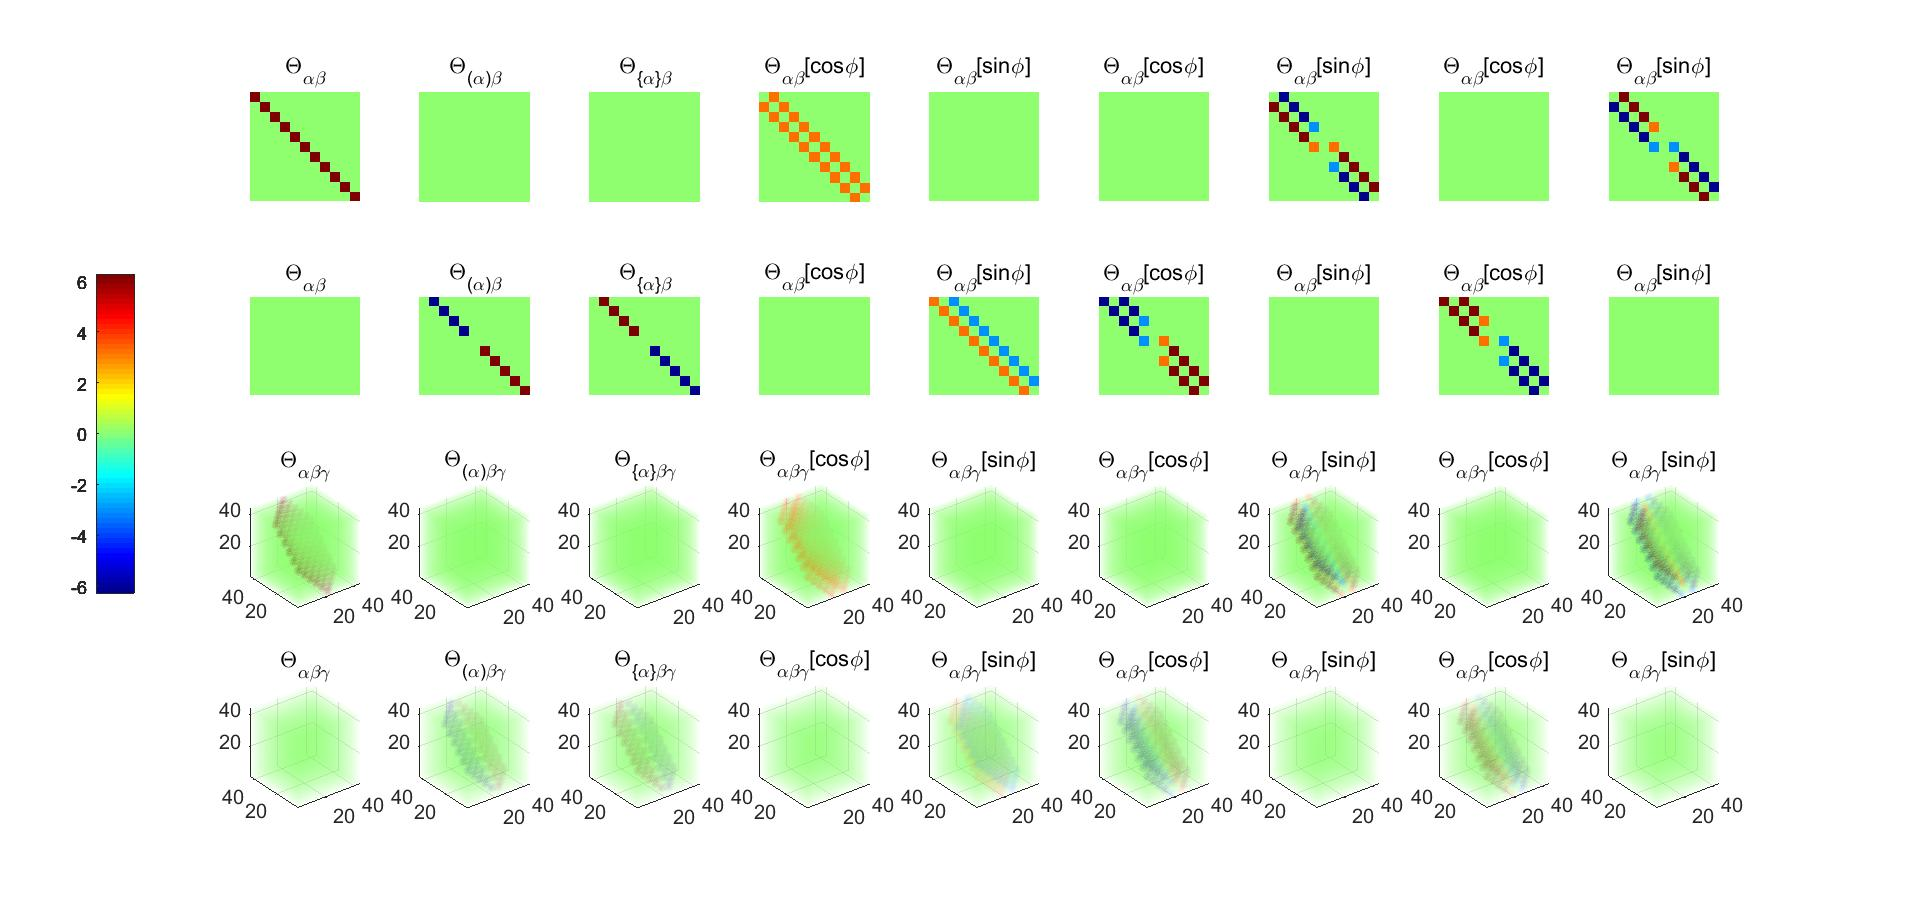
\includegraphics[width=8in]{ThetaFun.jpg}}
  \caption{$\Theta$}
  \end{figure}
  
  
  \subsection{Example for matlab simulation}
\begin{figure}
  \centerline{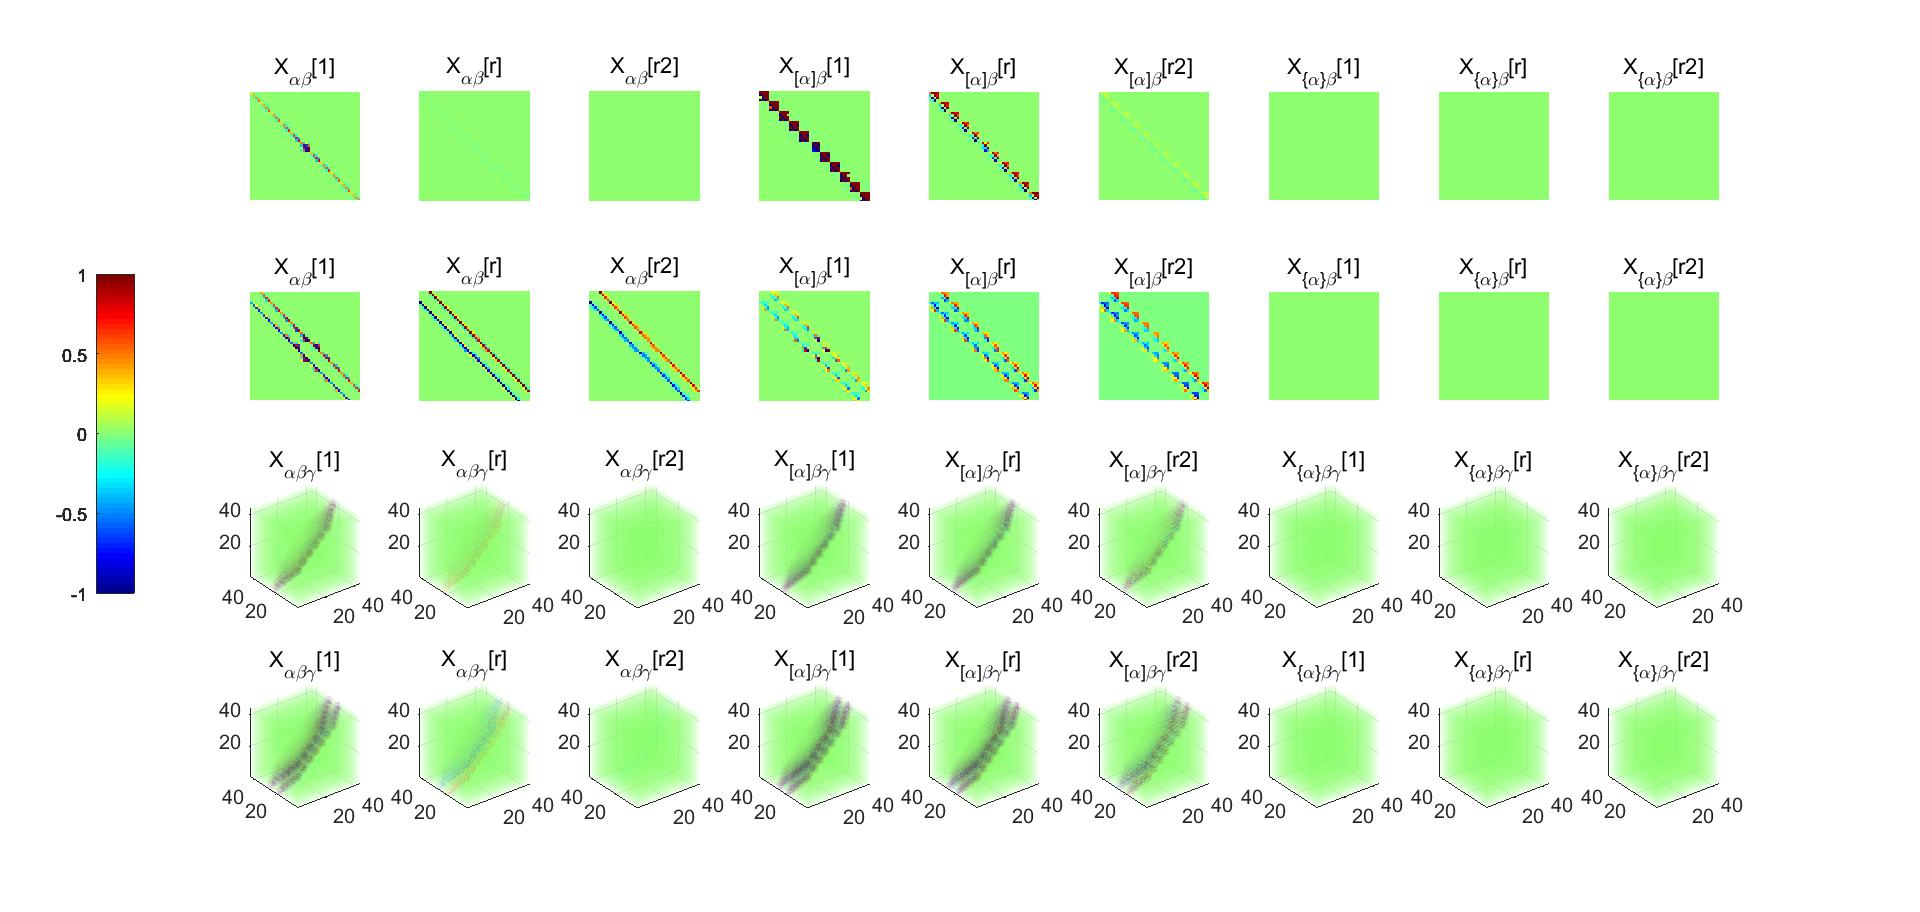
\includegraphics[width=8in]{XFun.jpg}}
  \caption{$X_ \Theta$}
  \end{figure}


  
  \subsection{Example for matlab simulation}
\begin{figure}
  \centerline{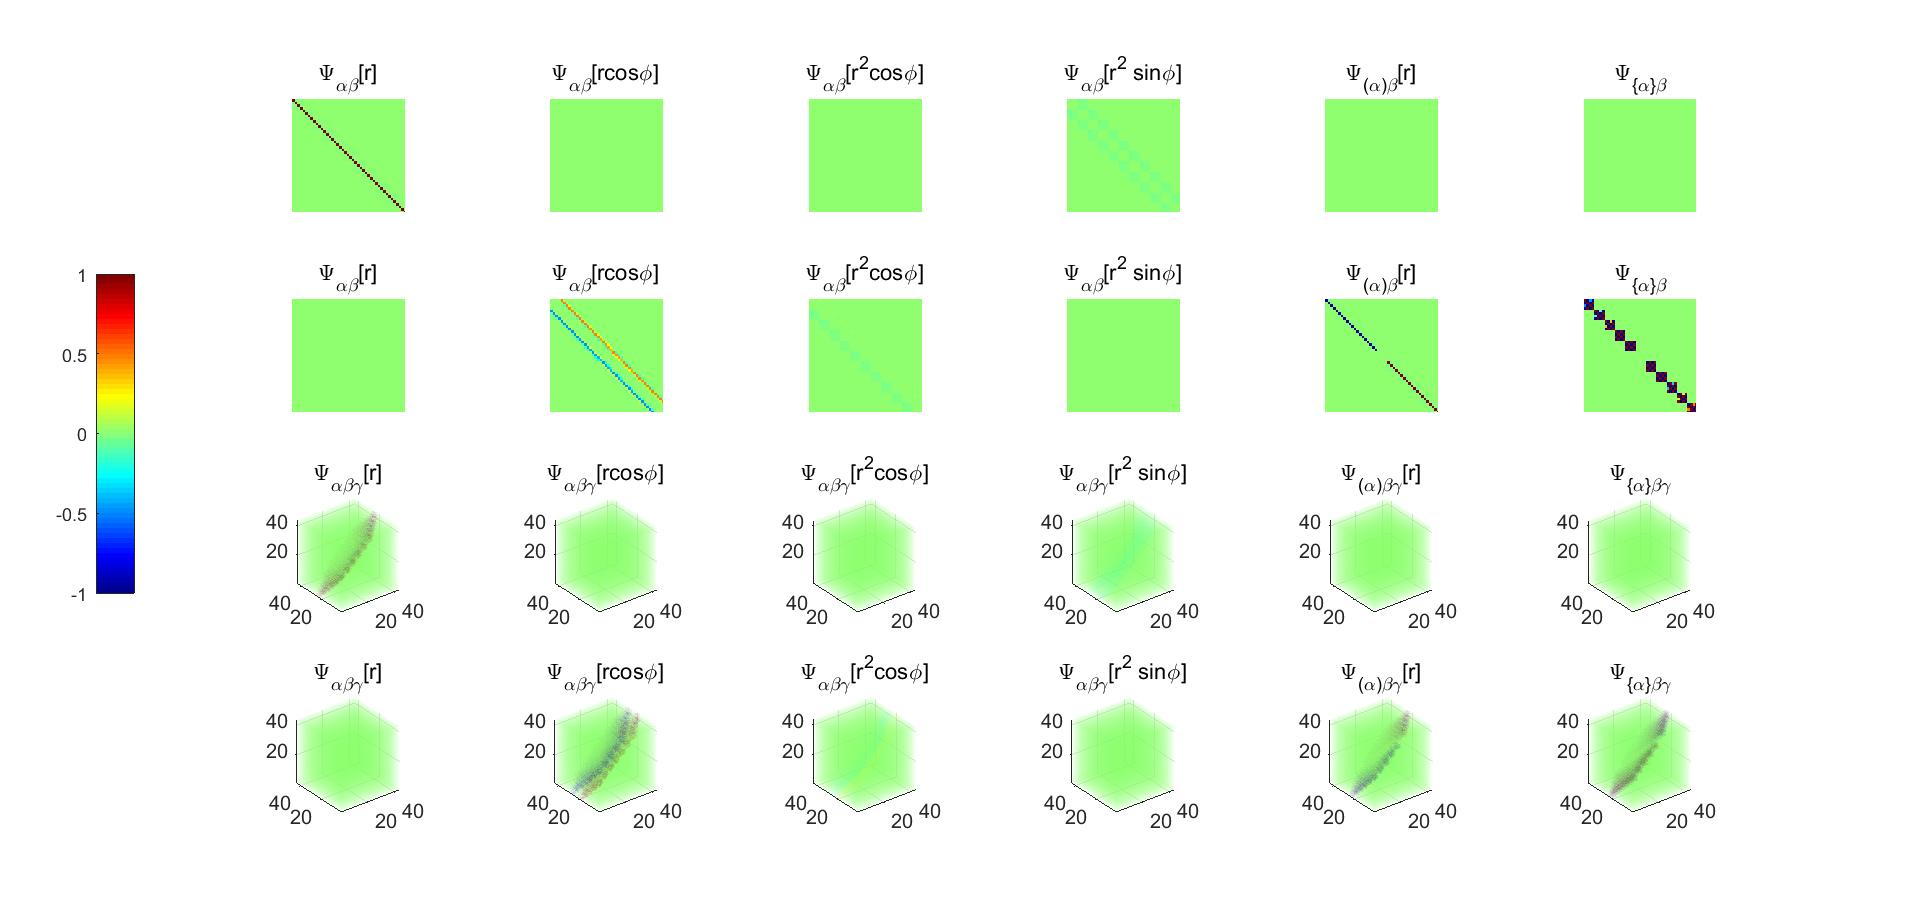
\includegraphics[width=8in]{PsiFun.jpg}}
  \caption{$\Psi$}
  \end{figure}





\begin{equation}
\begin{aligned}
Fig1:\Psi_{\alpha\beta}[r]=\mathcal{X}_{\alpha\beta}[r]\Theta_{\alpha\beta}:= \int_0^h r C_{\alpha_{mu}}(s) J_m({j'_{\alpha_{mu}}r\over h})  C_{\beta_{nv}} (scc)J_n({j'_{\beta_{nv}}r\over h})dr (2\pi \delta_{m,-n})\\
Fig2:  \Psi_{\alpha\beta}[rcos\phi]=\mathcal{X}_{\alpha\beta}[r]\Theta_{\alpha\beta}[cos\phi]:=
\int_0^h r C_{\alpha_{mu}} J_m({j'_{\alpha_{mu}}r\over h})  C_{\beta_{nv}} J_n({j'_{\beta_{nv}}r\over h})dr (\pi \delta_{m,-n-1}+\pi \delta_{m,-n+1})\\
 Fig3:  \Psi_{\alpha\beta}[r^2cos\phi]=\mathcal{X}_{\alpha\beta}[r^2]\Theta_{\alpha\beta}[cos\phi]:=
\int_0^h r^2 C_{\alpha_{mu}} J_m({j'_{\alpha_{mu}}r\over h})  C_{\beta_{nv}} J_n({j'_{\beta_{nv}}r\over h})dr  (\pi \delta_{m,-n-1}+\pi \delta_{m,-n+1})\\
 Fig4:  \Psi_{\alpha\beta}[r^2sins\phi]=\mathcal{X}_{\alpha\beta}[r^2]\Theta_{\alpha\beta}[sin\phi]:=
 \int_0^h r^2 C_{\alpha_{mu}} J_m({j'_{\alpha_{mu}}r\over h})  C_{\beta_{nv}} J_n({j'_{\beta_{nv}}r\over h})dr (-i(\pi \delta_{m,-n-1}-\pi \delta_{m,-n+1}))\\
  Fig5:  \Psi_{(\alpha)\beta}[r]=\mathcal{X}_{\alpha\beta}[r]\Theta_{(\alpha)\beta}:=
\int_0^h r C_{\alpha_{mu}} J_m({j'_{\alpha_{mu}}r\over h})  C_{\beta_{nv}} J_n({j'_{\beta_{nv}}r\over h})dr  (2\pi im \delta_{m,-n})\\
 Fig6:  \Psi_{\{\alpha\}\beta}=\mathcal{X}_{\{\alpha\}\beta}\Theta_{\alpha\beta}+\mathcal{X}_{\alpha\beta}\Theta_{\{\alpha\}\beta}\\
 \mathcal{X}_{\{\alpha\}\beta}:=-{h'\over h}(\mathcal{X}_{[\alpha]\beta}[r]+\mathcal{X}_{\alpha\beta})\\
 \mathcal{X}_{[\alpha]\beta}[r]:=\int_0^h r {d\over dr}(C_{\alpha_{m\mu}} J_m({j'_{\alpha_{m\mu}}r\over h}))C_{\beta_{nv}} J_n({j'_{\beta_{nv}}r\over h})dr\\
\Theta_{\{\alpha\}\beta}=\int_0^{2\pi} {\partial \over \partial s}(e^{im\phi}) e^{in\phi} d\theta
=-\tau 2\pi   im \delta_{m,-n}
\end{aligned}
\end{equation}





















\section{Tensors in matlab for numerical simulation}
\subsection{Tensor times vectors: $\mathcal{A}\bar{\times}_n u$}

Let $\mathcal{A}$ be a tensor of size $I_1\times I_2\times ...\times I_N$, u be a vector of size $I_n$.

We have:
\begin{equation}
\begin{aligned}
ttv(\mathcal{A},\{u\},[n])=(\mathcal{A}\bar{\times}_n u)(i_1,...,i_{n-1},i_{n+1},...,i_N)\\
\sum_{i_n=1}^{I_n}\mathcal{A}(i_1,i_2,...,i_N)u(i_n)
\end{aligned}
\end{equation}

\begin{equation}
\begin{aligned}
ttv(A_{m\times n},\{u_{m\times 1}\},[1])=A_{m\times n}\bar{\times}_1 u_{m\times 1}=A_{m\times n}^T u_{m\times 1}\\
ttv(A_{m\times n},\{v_{n\times 1}\},[2])=A_{m\times n}\bar{\times}_2 v_{n\times 1}=A_{m\times n}  v_{n\times 1}\\
\end{aligned}
\end{equation}

Property:

\begin{equation}
\begin{aligned}
ttv(\mathcal{A},\{u,v\},[m,n])=\mathcal{A}\bar{\times}_m u \bar{\times}_n v\\
=ttv(ttv(\mathcal{A},\{u\},[m]),\{v\},[n-1])=(\mathcal{A}\bar{\times}_m u ) \bar{\times}_{n-1} v\\
=ttv(ttv(\mathcal{A},\{v\},[v]),\{u\},[m])=(\mathcal{A}\bar{\times}_n v ) \bar{\times}_{m} u\\
\end{aligned}
\end{equation}

Multiplication with a sequence of vectors
\begin{equation}
\begin{aligned}
\beta=\mathcal{A}\bar{\times}_1 u^{(1)}\bar{\times}_2 u^{(2)}...\bar{\times}_N u^{(N)}=\mathcal{A}\bar{\times} {u}\\
like:
ttv(X, \{A,B,C,D\})
= ttv(X, \{A,B,C,D\}, [1 2 3 4]) 
= ttv(X, \{D,C,B,A\}, [4 3 2 1])
\end{aligned}
\end{equation}

Multiplication with \textbf{all but one} of a sequence of vectors
\begin{equation}
\begin{aligned}
b=\mathcal{A}\bar{\times}_1 u^{(1)}\bar{\times}_2 u^{(2)}...\bar{\times}_{n-1} u^{(2)}\bar{\times}_{n+1} u^{(2)}...\bar{\times}_N u^{(N)}=\mathcal{A}\bar{\times}_{-n} {u}\\
like:
X = tenrand([5,3,4,2]); \\
A = rand(5,1); B = rand(3,1); C = rand(4,1); D = rand(2,1); \\
Y = ttv(X, \{A,B,D\}, -3) = ttv(X, \{A,B,C,D\}, -3)
\end{aligned}
\end{equation}

\subsection{Tensor times matrix (ttm): $\mathcal{A}{\times}_n u$}
Let $\mathcal{A}$ be a tensor of size $I_1\times I_2\times ...\times I_N$, U be a matrix of size $J_n\times I_n$.

We have:
\begin{equation}
\begin{aligned}
ttm(\mathcal{A},\{U\},[n])=(\mathcal{A}{\times}_n U)(i_1,...,i_{n-1},j_{n},i_{n+1},...,i_N)\\
\sum_{i_n=1}^{I_n}\mathcal{A}(i_1,i_2,...,i_N)U(j_n, i_n)\\
like:X = tensor(rand(5,3,4,2));
A = rand(4,5);\\
Y = ttm(X, A, 1)= ttm(X, \{A,B,C,D\}, 1)= ttm(X, A', 1, 't')    
\end{aligned}
\end{equation}

Matrix Interpretation
\begin{equation}
\begin{aligned}
ttm(A_{m\times n},\{U_{m\times k}^T\},[1])=A\times _1 U^T=U^TA\\
ttm(A_{m\times n},\{V_{m\times k}^T\},[2])=A\times _2 V^T=AV\\
ttm(A,\{U,V\},[1,2])=UAV^T
\end{aligned}
\end{equation}

\begin{equation}
\begin{aligned}
Y = ttm(X, {A,B,C,D}, [1 2 3 4]); \%<-- 4-way mutliply.\\
Y = ttm(X, {D,C,B,A}, [4 3 2 1]); \%<-- Same as above.\\
Y = ttm(X, {A,B,C,D});            \%<-- Same as above.\\
Y = ttm(X, {A',B',C',D'}, 't')    \%<-- Same as above.\\
\\
Y = ttm(X, {C,D}, [3 4]);    \%<-- X times C in mode-3 & D in mode-4\\
Y = ttm(X, {A,B,C,D}, [3 4]) \%<-- Same as above.\\
\\
Y = ttm(X, {A,B,D}, [1 2 4]);  \%<-- 3-way multiply.\\
Y = ttm(X, {A,B,C,D}, [1 2 4]); \%<-- Same as above.\\
Y = ttm(X, {A,B,D}, -3);        \%<-- Same as above.\\
Y = ttm(X, {A,B,C,D}, -3)       \%<-- Same as above.\\
\end{aligned}
\end{equation}


Property
\begin{equation}
\begin{aligned}
ttm(\mathcal{A},\{u,v\},[m,n])=\mathcal{A}{\times}_m u \bar{\times}_n v\\
=ttm(ttm(\mathcal{A},\{u\},[m]),\{v\},[n])=(\mathcal{A}{\times}_m u ){\times}_{n} v\\
=ttm(ttm(\mathcal{A},\{v\},[v]),\{u\},[m])=(\mathcal{A}{\times}_n v ) {\times}_{m} u\\
\end{aligned}
\end{equation}


\subsection{Tensor times tensor (ttt): $<\mathcal{A},\mathcal{B}>$}
Let $\mathcal{A}$ and $\mathcal{B}$ be a tensor of size $I_1\times I_2\times ...\times I_N$.
\begin{equation}
\begin{aligned}
<\mathcal{A},\mathcal{B}>=\\
\beta=\sum_{i_1=1}^{I_1}\sum_{i_1=1}^{I_2}...\sum_{i_1=1}^{I_N}\mathcal{A}(i_1,i_2,...,i_N)\mathcal{B}(i_1,i_2,...,i_N)
\end{aligned}
\end{equation}

\begin{equation}
\begin{aligned}
X = tensor(rand(4,2,3)); Y = tensor(rand(3,4,2));\\
Z = ttt(X,Y); \%<-- Outer product of X and Y.\\
size(Z)\\
\\
Z = ttt(X,X,1:3) \%<-- Inner product of X with itself.\\
\\
Z = ttt(X,Y,[1 2 3],[2 3 1]) \%<-- Inner product of X & Y.\\
\\
Z = innerprod(X,permute(Y, [2 3 1])) \%<-- Same as above.\\
\\
Z = ttt(X,Y,[1 3],[2 1]) \%<-- Product of X & Y along specified dims.\\
\end{aligned}
\end{equation}


\section{model of helical duct}
\subsection{w}

The duct is described by its centreline $\textbf{q}(s)$ at arclength s from the inlet of the duct adn the radial distance from the centreline $h=h(s)$. The general position vector $\textbf(x)$ in the duct is given in terms of $(s,r,\theta)$:

\begin{equation}
\begin{aligned}
\textbf{x}=\textbf{q}(s)+rcos(\theta-\theta_0) \widehat{\textbf{n}}+rsin(\theta-\theta_0) \widehat{\textbf{b}}
\end{aligned}
\end{equation}

where $\widehat{\textbf{n}}=\widehat{\textbf{n}}(s)$ is the normal to the centreline and $\widehat{\textbf{b}}=\widehat{\textbf{b}}(s)$ id the binormal given by $\widehat{\textbf{b}}=\widehat{\textbf{t}}\times \widehat{\textbf{n}}$ for the tangent to the centreline $\widehat{\textbf{t}}=\widehat{\textbf{t}}(s)$. The vector $\widehat{\textbf{n}}$,$\widehat{\textbf{b}}$ and $\widehat{\textbf{t}}$ are related by the Frenet-Serret formulas:
\begin{equation}
\begin{aligned}
{d\widehat{\textbf{q}}\over ds}=\widehat{\textbf{t}},\quad {d\widehat{\textbf{t}}\over ds}=\kappa \widehat{\textbf{n}},\quad {d\widehat{\textbf{n}}\over ds}=-\kappa \widehat{\textbf{t}}+\tau \widehat{\textbf{b}},\quad {d\widehat{\textbf{b}}\over ds}=-\tau \widehat{\textbf{n}}
\end{aligned}
\end{equation}

where $\kappa=\kappa(s)$ is the local curvature of the duct and $\tau=tau(s)$ is the torsion. Here, intorduce $\theta_0'=\tau$, the cross-term differentials vanish and the metric reduces:
\begin{equation}
\begin{aligned}
d\textbf{x}=d(\textbf{q}(s))+d(rcos(\theta-\theta_0) \widehat{\textbf{n}})+d(rsin(\theta-\theta_0)\widehat{\textbf{b}})\\
=\widehat{\textbf{t}}ds +dr cos\phi \widehat{\textbf{n}}-r\widehat{\textbf{n}} sin\phi (d\theta-\tau ds)+r cos\phi (-\kappa \widehat{\textbf{t}}+\tau \widehat{\textbf{b}})ds\\
+dr sin\phi \widehat{\textbf{b}}+r\widehat{\textbf{b}} cos\phi (d\theta-\tau ds)+r sin\phi (-\tau \widehat{\textbf{n}})ds\\
=\widehat{\textbf{t}}(1-\kappa r cos\phi)ds+\widehat{\textbf{n}}(dr cos\phi-rsin\phi d\theta)+\widehat{\textbf{b}}(dr sin\phi+rcos\phi d\theta)
\end{aligned}
\end{equation}

Thus,
\begin{equation}
\begin{aligned}
d\textbf{x}\cdot d\textbf{x}
={(1-\kappa r cos\phi)}^2ds^2+{(dr cos\phi-rsin\phi d\theta)}^2+{(dr sin\phi+rcos\phi d\theta)}^2\\
={(1-\kappa r cos\phi)}^2ds^2+dr^2+r^2d\theta
\end{aligned}
\end{equation}

As a result, we have an orthogonal coordinate system and as such do not need to distinguish between covariant and contravariant bases.






\section{funm-Evaluate general matrix function}

https://ww2.mathworks.cn/help/matlab/ref/funm.html















\end{document}


